% PREAMBLE

\documentclass[12pt]{scrreprt}

\usepackage[a4paper]{geometry}
\usepackage{graphicx,color}
\usepackage[numbers,sort&compress]{natbib}
\usepackage[utf8]{inputenc}
\usepackage[ngerman]{babel}
\usepackage{amsmath,amssymb}
\usepackage{amsthm,mathdots,gauss}

\usepackage{pxfonts}

\usepackage{hyperref,float,bbding,stmaryrd}

% amsthm conf
\newtheorem{definition}{Definition}
\newtheorem{theorem}{Satz}
\newtheorem{lemma}{Lemma}
\newtheorem{example}{Beispiel}
\newtheorem{note}{Anmerkung}
\newtheorem{proposition}{Behauptung}

% tikz, geogebra colors
\usepackage{pgf,tikz}
\usetikzlibrary{arrows}
% geogebra farbcodes unschoen, aber zu aufwendig um die haendisch auszubessern -.-
\definecolor{qqqqff}{rgb}{0,0,1}
\definecolor{xdxdff}{rgb}{0.49,0.49,1}
\definecolor{uququq}{rgb}{0.25,0.25,0.25}
\definecolor{evtftf}{rgb}{0.9,0.25,0.25}
\definecolor{qqqqff}{rgb}{0,0,1}
\definecolor{qqwuqq}{rgb}{0,0.39,0}
\definecolor{qqffqc}{rgb}{0,1,0.05}


% macros
\newcommand{\lecture}[1]{


  \noindent
  \fbox{
      \begin{minipage}{\textwidth}\centering
        \textbf{Vorlesung vom #1}
      \end{minipage}
  }
}

% Style
\renewcommand{\theenumi}{\arabic{enumi}}
\renewcommand{\labelenumi}{(\theenumi)}
\renewcommand{\theenumii}{\alph{enumii}}
\renewcommand{\labelenumii}{(\theenumii)}
\allowdisplaybreaks

% Meta
\title{Analysis für Informatiker}
\author{Lars Hupel\\ Michael Kerscher\\ Markus Grimm\\ Andreas Heider}
\date{\today}

% Lecturer shortcuts
\newcommand{\induction}{Beweis per vollständiger Induktion \Checkmark}
\newcommand{\imag}{\operatorname{i}}
\newcommand{\euler}{\operatorname{e}}
\newcommand{\equals}{\stackrel{\scriptscriptstyle\wedge}{=}}



%%% meta

\title{Analysis für Informatiker}
\author{Lars Hupel\\ Michael Kerscher\\ Markus Grimm\\ Andreas Heider \\ Janosch Peters}
\date{\today}

\begin{document}

\maketitle

\newpage
\listoftodos
\newpage
\tableofcontents
\newpage
\addcontentsline{toc}{chapter}{Vorlesungsverzeichnis}
\listoflectures
\newpage

\chapter{Grundlagen: Zahlbegriff}

\lecture{2009-10-20}


\section{Zahldarstellung}
\subsection{Natürliche Zahlen zu reelle Zahlen}
diskret: $1,2,3,...$\\
$\mathbb{N} = \{1,2,3,...\}$ Menge der natürlichen Zahlen
\begin{definition}
 Menge ist Zusammenfassung bestimmter wohlunterschiedener Objekte unserer Anschauung oder unserers Denkens
\end{definition}

\subsubsection*{Axiomensystem nach Peano}
\begin{enumerate}
 \item $1 \in \mathbb{N}$ (Anfang)
 \item $n \in \mathbb{N} \Rightarrow (n+1) \in \mathbb{N}$ (Nachfolger)
 \item $n \neq m \Rightarrow (n+1) \neq (m+1)$
 \item $n \in \mathbb{N} \Rightarrow (n+1) \neq 1$
 \item $A \in \mathbb{N}: 1 \in A \land (\forall n: n \in A \Rightarrow (n+1) \in A) \Rightarrow A = \mathbb{N}$ (Vollständigkeitsaxiom, alle natürlichen Zahlen werden erfasst)
\end{enumerate}

\subsubsection*{Erweiterungen}

\begin{enumerate}
 \item ...zu $\mathbb{Z} = \{\ldots,-2,-1,0,1,2,\ldots\}$ ganze Zahlen. In $\mathbb{Z}$ Operationen $+,-$
 \item ...zu $\mathbb{Q}$ rationale Zahlen durch $*,/$, $q=\frac{m}{n}; m \in \mathbb{Z}, n \in \mathbb{N}$
  \begin{equation*}\mathbb{Q} = \left\{x | x=\frac{m}{n}, m \in \mathbb{Z}, n \in \mathbb{N} \right\}\end{equation*}
  $\mathbb{Q}$ ist dicht, d.h. zwischen $q_1, q_2$ liegt ein $\tilde{q}$
 \item ...durch $\sqrt{}$ (Wurzelziehen) bzw. Quadrieren $x^2=a$
 \begin{equation*}a=2 \Rightarrow x = \sqrt{a} \notin \mathbb{Q}, \sqrt{2}=1,4142\ldots\text{ irrational}\end{equation*}

\begin{proof}[Beweis (indirekt)]
Aus $\sqrt{2} \in \mathbb{Q} \Rightarrow \sqrt{2}=\frac{p}{q}$ gekürzt ($p \in \mathbb{Z}, g \in \mathbb{N}$
$2g^2=p^2 \Rightarrow p^2$ gerade $\Rightarrow p=2\hat{p}$ und $2g^2=4\hat{p}^2$
$\Rightarrow g^2 = 2\hat{p}^2 \Rightarrow g=2\hat{g}$ 
$\Rightarrow$ Widerspruch zur gekürzten Form: $\sqrt{2}=\frac{p}{q}=\frac{2\hat{p}}{2\hat{g}}$

Aussage: $\sqrt{2}$ ist keine rationale Zahl.
\end{proof}

Beweistechnik war indirekt, z. z. Aussage $A$ $\Rightarrow$ Aussage $B$\\
indirekt: "`nicht"' Aussage $B$ $\Rightarrow$ "`nicht"' Aussage $A$


\begin{proof}[Beispiel: direkte Beweistechnik]

$p \in \mathbb{N}$ gerade $\Leftrightarrow p = 2 \hat{p} \Leftrightarrow p^2 = 4\hat{p}^2$ gerade\\
$p \in \mathbb{N}$ ungerade $\Leftrightarrow p = 2 \hat{p}+1 \Leftrightarrow p^2 = (2\hat{p}+1)^2=4\hat{p}^2+4\hat{p}+1$ ungerade\\
$\Rightarrow$ reelle Zahlen, formaler Weg siehe \cite[S. 9ff]{bornemann}
\end{proof}

 \item reelle Zahlen -- neue Kandidaten im Vergleich zu $\mathbb{Q}$
\begin{itemize}
 \item $\sqrt{}$-Bildung
 \item $c = 0,\overline{b_1 \;\ldots\; b_k}$ periodische Zahl\\
$c = \cfrac{b_1 \;\ldots\; b_k}{\underbrace{g \;\ldots\; g}_{k\text{-mal}}} \in \mathbb{Q} \Rightarrow 10^k c -c = b_1 \ldots b_k$ periodischer Bruch\\
(eine neue periodische Zahl, die nicht als Bruch darstellbar ist, wäre z. B. $c=0,101001000100001\ldots$)
 \item $\infty$-Summen, $\euler, \pi,\ldots$
\end{itemize}

\end{enumerate}

\subsection{Maschinenzahlen $\mathbb{M}$}
\integer-Zahlen (Assoziation: $\mathbb{Z}$), \real-Zahlen (Assoziation: $\mathbb{R})$ sind 2 Typen unterschiedlicher Codierung

4 Byte für \integer; 4, 8, 10 Byte für \real

\subsubsection*{\integer}

31 Bits für Mantisse, größte Zahl $\pm \underbrace{1\ldots1}_{31\text{ Mal}}$ (im Zweiersystem)

entspricht Zahldarstellung: $2^0+2^1+\ldots+2^{30}=2^{31}-1$ \\
$\leadsto$ 10er-System: $2^{31}-1 \equals x$, $2^{10}\approx 10^3$\\
Zahlbereich: -2 Mrd. bis 2 Mrd

\subsubsection*{\real-4}

Mantisse 23 Bits, Exponent 7 Bits

$\pm 0.\underbrace{\text{\ttfamily\_\_\_\_\_}\ldots\text{\ttfamily\_\_\_\_\_}}_{\text{Mantisse}}e\pm\underbrace{\text{\ttfamily\_\_\_}\ldots\text{\ttfamily\_\_\_}}_{\text{Exponent}}$

Darstellung ist \emph{normalisiert}, d. h. nach Dezimalpunkt keine Nullen (IEEE 754 $\hat{=}$ VDE)

\begin{itemize}
 \item Exponentenspielraum: $1\cdot 2^0+1\cdot2^1+\ldots+1\cdot2^6 = 2^7 -1 = 127$
  Exponent $10^{-127}$ bis $10^{127}$
 \item Länge der Maschine im 10er-System:\\
$1\cdot 2^0+1\cdot2^1+\ldots+1\cdot2^22=2^{23} \equals 10^x$\\
$2^{23}\equals 10^x, x=23 \log_{10}(2) \approx 6,923 $ \todo{soll das hier stehen?}\\
$m \in \mathbb{M}, m=\pm 0.\text{\ttfamily\_\_\_\_\_}\ldots\text{\ttfamily\_\_\_\_\_} e\pm \text{\ttfamily\_\_\_}\ldots\text{\ttfamily\_\_\_}$\\Lücke zwischen $-10^{-127}$ und $10^{-127}$ Faktor $10^7$ groß
\end{itemize}

\subsubsection{Rundungsfehler}

Wesentlich mitbestimmt von F. L. Bauer, Samelson, Zenger aus der Informatik und R. Bukisch und Chr. Reinsch aus der Mathematik und Wilkinson.\\
Hilfsmittel: Abbildung von den reellen Zahlen (Alltag) auf den Rechner

\begin{definition}[Abbildung \emph{rd} bzw. \emph{round} (Rundung)]
rd: $\mathbb{R}\rightarrow\mathbb{M}$\\
rd: $\left\{x|x \in [\frac{m_{i-1}+m_i}{2},\frac{m_{i}+m_{i+1}}{2}[\right\} \mapsto m_i$
\end{definition}

\begin{note}
Intervall-Arithmetik hat sich trotz Hardwareunterstützung nicht bewährt: Intervallängen zu pessimistisch.
\end{note}

\begin{definition}[Abbildung]
Vorraussetzung: $A$, $B$ Mengen\todo{prüfen}
\begin{equation}f: A \rightarrow B, x \mapsto f(x)\end{equation}
Eine Abbildung ist eine Vorschrift, die jedem $x \in A$ ein Element $x=f(x) \in B$ zuordnet.
\end{definition}

\subsubsection*{Charakterisierung von Abbildungen}
\begin{itemize}
 \item gehören zu verschiedenen Argumenten verschiedene Funktionswerte, heißt $f$ \emph{injektiv:}
\[\forall x_1,x_2 \in A: x_1 \neq x_2 \Rightarrow f(x_1) \neq f(x_2)\]
 \item Wertebereich $C \subseteq A$:
\[ f(C) = \{f(x)|x\in C\} \]
 \item $f$ \emph{surjektiv}, falls $f(A)=B$
 \item $f$ injektiv und surjektiv $\Leftrightarrow$ $f$ \emph{bijektiv}

$f: A \mapsto B$ ist genau dann bijektiv, falls zu jedem $y \in B$ genau ein $x \in A $ existiert mit $y=f(x)$. In diesem Fall existiert eine Umkehrabbildung $f^{-1}: B \mapsto A$.
\end{itemize}

\lecture{2009-10-21}

\subsection{Ungleichungen,  Betrag Kalkül-Teil}
Definition: Unter einer Ungleichung für reelle Zahlen $x,y$ verstehen wir einen Größenvergleich
\begin{center}
% use packages: array
\begin{tabular}{lll}
$x<y$ & "kleiner $<$" & kleiner $\leq$ \\ 
$x>y$ & "größer $>$" & größer $\geq$
\end{tabular}
\end{center}

Abschätzung: $x<y$ heißt Größe von $x$ durch Größe von $y$ abschätzen. Regelwerk für Abschätzungen (Anordnungsaxiome)
$\leadsto$ Zahlengerade.
\begin{enumerate}
 \item $x \leq y, a\leq b \Rightarrow x+a \leq y+b$
 \item $x<y, 0 \leq a \Rightarrow ax \leq ay$
 
$x<y, 0 < a \Rightarrow ax < ay$
 \item $0<x\leq y \Rightarrow 0 < \frac{1}{y} \leq \frac{1}{x}$
\end{enumerate}
Typische Aufgabe:
lege $a$ fest mit Eigenschaft
\begin{align*}
-3a-2 &\leq 5 &\leq -3a+4 \\
-3a\leq 7 & & 1 \leq -3a \\
-\frac{1}{3} &\leq a &\leq -\frac{7}{3}
\end{align*}

Definition: $S \subset \mathbb{R}$ heißt nach oben beschränkt, falls eine Zahl $b$ existiert mit $S\subseteq ]-\infty,b]$ "b obere Schranke von S"

Definition: Ist $S \subseteq \mathbb{R}$ nach oben beschränkt, so heißt die kleinste obere Schranke von $S$ das \emph{Supremum} $s:=\sup S$

analog: \emph{Infimum}: "größte unter Schranke" $u := \inf S$

Bemerkung: kleinste obere Schranke muss nicht element von $S$ sein, das \emph{Maximum} schon

\begin{itemize}
 \item $\sup \{x \in \mathbb{Q} | x^2 < 2 \} = \sqrt{2} \notin \mathbb{Q}$
 \item $\sup \{[a,b]\} = b \in [a,b]$
 \item $\inf \{ 1+\frac{1}{n}|n\in \mathbb{N}\} = 1$
\end{itemize}

Vollständigkeitsaxiom für $\mathbb{R}$
Jede nach oben beschränkte Menge reeller Zahlen besitzt ein \emph{Supremum}.$\mathbb{R}$ überabzählbar, $\mathbb{Q}$ abzählbar (siehe Bornemann)

Definition: Betrag $|a|, a \in \mathbb{R}$
$|a|=a \textrm{falls} a \geq 0 \land -a \textrm{falls} a<0$

Rechenregeln(Beträge):
\begin{itemize}
 \item $-|a|\leq a \leq |a|$
 \item $-|a| = |a|$
 \item $|ab| = |a||b|$
 \item $|\frac{a}{b}| = \frac{|a|}{|b|}, b\neq 0$
\end{itemize}

Anwendung: Dreiecksungleichung
z.z.: $|a+b| \leq |a|+|b|$. Dazu
\begin{align*}
-|a|&\leq a &\leq |a| \\
-|b|&\leq b &\leq |b| \\
\Rightarrow -(|a|+|b|)&\leq a+b &\leq |a|+|b| \\
-(|a|+|b|)&\leq |a+b| &\leq |a|+|b|
\end{align*}
Abstandsmessung $|x-a| \leq \epsilon$

Rechenbeispiel:
$x\in \mathbb{R}$ gesucht mit $\frac{3}{x-9} \leq \frac{2}{x+2}$. Nenner $x\neq9 \land x\neq -2$

(Zahlenstrahl mit Markierung von -2 nach links und Markierung von 9 nach rechts)

\begin{align*}
M_1 &= \{x \in \mathbb{R} | x < -2\} \\
M_2 &= \{x \in \mathbb{R} | -2 < x < 9\} \\
M_3 &= \{x \in \mathbb{R} | x > 9\}
\end{align*}

\begin{itemize}
 \item Diskussion von $M_1: x < -2$
\begin{align*}
|x-9|>0 &\Rightarrow \frac{3}{|x-9|} > 0 \\
x<-2 &\Rightarrow x+2<0 \Rightarrow \frac{2}{x+2}<0
\end{align*}
ganz $M_1$ zulässig
 \item Diskussion von $M_2: -2<x<9$
\begin{align*}
\Rightarrow &x+2 > 0 \\
&x-9<0 \textrm{d.h.} |x-9|=9-x \\
\textrm{zu prüfen:}
\frac{3}{9-x} > \frac{2}{x+2} \textrm{Betrag weg} \\
3x+6 > 18-2x \\
x > \frac{12}{5} = 2 \frac{2}{5}
\textrm{erlaubt:} \frac{12}{5}<x<9
\end{align*}
 \item Diskussion von $M_3: x>9$
\begin{align*}
 \Rightarrow \underbrace{|x-9|}_{>0} = x-9 \\
\frac{3}{x-9} > \frac{2}{x+2}
\Rightarrow x>-24
\end{align*}
$M_3$ zulässig

Ergebnis: $\{x|x<-2, \frac{12}{5}<x<9, 9<x\}$
\end{itemize}

Anwendung: Geometrie
\begin{align*}
M = \{(x,y)| |x|+|y| \leq 1 \} x,y \in \mathbb{R} \\
|x|+|y| \leq 1 \Rightarrow &x \geq 0, y \geq 0: x+y \leq 1 \Rightarrow y \leq 1-x \\
	&x \geq 0, y < 0: x-y \leq 1 \Rightarrow y \geq -1+x \\
	&x < 0, y \geq 0: -x+y \leq 1 \Rightarrow y \leq 1+x \\
	&x < 0, y < 0: -x-y \leq 1 \Rightarrow y \geq -1-x \\
\end{align*}
(Zeichnung einer "Raute" mit gefülltem Inhalt als Lösung)

Kreis um Ursprung mit Fläche
Radius $\{(x,y)| x^2+y^2\leq r^2 \}$

Kreislinie $\{(x,y)| x^2+y^2 = r^2 \}$

\lecture{2009-10-27}

\section{Vollständige Induktion}

bisherige Beweistechniken:

\begin{enumerate}
 \item direkter Beweis: $A \Rightarrow B$
 \item indirekter Beweis: $\neg B \Rightarrow \neg A$
\end{enumerate}
jetzt: vollständige Induktion

\subsection{Schema}

\begin{enumerate}
 \item Induktionsbeginn (bzw. -anfang): zeige, dass Aussage $A(n)$ für ein festes $n_0 \in \mathbb{N}$ gilt
 \item Induktionsschluss: $A(n)$ zu $A(n+1)$
\end{enumerate}

\begin{example}
 \begin{itemize}
  \item $1+2+\ldots+n = \frac n 2 (n+1)$
    \begin{enumerate}
    \item Induktionsanfang: $n_0 = 1$, $1 = \frac 1 2 (1+1) = 1$
    \item Induktionsschluss: \begin{equation*}\underbrace{1+2+\ldots+n}_{A_n} + (n+1) = \frac 1 2 (n+1) + (n+1) = \frac{n+1}2 (n+2)\end{equation*}
    \end{enumerate}
  \item $1^2+2^2+\ldots+n^2 > \frac{n^3}3$
    \begin{align*}
      n_0 = 1:\text{\hspace{1cm}} &1 > \frac 1 3 \text{\hspace{1cm}} \\
      n \rightarrow n + 1 :\text{\hspace{1cm}} &\underbrace{1^2+2^2+\ldots+n^2}_{>\frac{n^3}3}+(n+1)^2 > \frac{n^3}3+(n+1)^2 \\
      &= \frac{n^3+3n^2+6n+3}3 > \frac{n^3+3n^2+3n+1}3 = \frac{(n+1)^3}3
    \end{align*}
 \end{itemize}
\end{example}

Eng verwandt mit der vollständigen Induktion ist die Rekursion:
\begin{itemize}
 \item lege $A_0$ fest
 \item setze $A_k$ als bekannt voraus für $k \leq n$
 \item definiere $A_n$ aus $A_k$
\end{itemize}

\begin{example}[Standard]
  \begin{itemize}
    \item Potenz: $a \in \mathbb{R}, n \in \mathbb{N}: a^0 = 1, a^{n+1} = a\cdot a^n$
    \item Fakultät: $n \in \mathbb{N}_0:$
    \begin{equation*} n! = \begin{cases} 1 & n = 0 \\ n \cdot (n-1)! & n \geq 1 \end{cases} \end{equation*}
  \end{itemize}
\end{example}

\begin{definition}[Summensymbol]
  \begin{equation*} a_j \in \mathbb{R}: a_0 + a_1 + \ldots + a_n =: \sum_{j=0}^{n} \left( a_j \right) \end{equation*}
\end{definition}

\subsection{Potenzen, Wurzel}

\begin{theorem}[Satz zur $m$-ten Potenz]\flush
  $x,y \in \mathbb{R}; n,m \in \mathbb{N}_0$
  \begin{enumerate}
   \item $x^nx^m = x^{n+m}$
   \item $(x^n)^m = x^{nm}$
   \item $(xy)^n = x^ny^n$
   \item $y \neq 0 \Rightarrow \left(\frac x y\right)^n = \frac{x^n}{y^n}$
   \item $0 < x < y \Rightarrow 0 < x^n < y^n$
   \item $n \geq 2, 0<x<1 \Rightarrow x^n<x<1$
   \item $n \geq 2, x > 1 \Rightarrow x^n>x>1$
   \item $x > 1, m > n \Rightarrow x^m > x^n$
  \end{enumerate}
  (\induction)
\end{theorem}
%
\noindent Hilfsmittel für Abschätzungen: Linearisierungen, Bernoulli-Ungleichung

\begin{proposition}
  für alle $x > -1, x \neq 0$ und $n \in \mathbb{N}, n \geq 2$ gilt
  \begin{equation*} \underbrace{(1+x)^n}_\text{nichtlin. Term} > \underbrace{1+nx}_\text{lin. Term} \end{equation*}
  \induction
\end{proposition}
%
Wunsch: in der Nähe von 1, d. h. $1+x$ für kleine $x$, soll der lineare Term den nichtlinearen Term ersetzen (Abschätzungstechnik)

\begin{theorem}[Elementare Summenformel]\flush
 $q \in \mathbb{R}, n \in \mathbb{N}$
 \begin{equation*} \sum_{k=0}^n \left( q^k\right) = \begin{cases}\frac{1-q^{n+1}}{1-q} & q \neq 1 \\ n+1 & q = 1\end{cases} \end{equation*}
\end{theorem}

\induction

\begin{definition}[$n$-te Wurzel]\flush
 $x\in \mathbb{R}$
 \begin{align*}
  x \geq 0,\; n \text{ gerade} &\Rightarrow \exists_{y \in \mathbb{R}} \left( y >= 0 \Rightarrow y^n = x \right) \\
  x \text{ bel.},\; n \text{ ungerade} &\Rightarrow \exists_{y \in \mathbb{R}} \left( y^n = x \right) \\
 \end{align*}
Bezeichnung: $y = \sqrt[n]{x} = x^\frac 1 n$\\
Problem: $\sqrt{-1}$ sprengt $\mathbb{R}$, Definition der imaginären Einheit $\imag$\\$\leadsto$ komplexe Zahlen $\mathbb{C}$ (später)
\end{definition}

\subsubsection*{Rechenregeln für Wurzeln}

$x,y \in \mathbb{R}$ passend zu $n,m \in\mathbb{N}$
\begin{enumerate}
 \item $\sqrt[n]{xy} = \sqrt[n]x \sqrt[n]y$
 \item $\sqrt[n]{\sqrt[m]x} = \sqrt[nm]x$
 \item $\sqrt[n]{x^m} = (\sqrt[n]x)^m$
 \item $x<y \Rightarrow \sqrt[n]x < \sqrt[n]y$
 \item $0<x<1, m<n \Rightarrow \sqrt[m]{x} < \sqrt[n]{x}$
 \item $x>1, m<n \Rightarrow \sqrt[m]x > \sqrt[n]x$
 \item $\sqrt[n]{x^n} = \begin{cases} x & n \text{ ungerade} \\ |x| & n \text{ gerade} \end{cases}$
\end{enumerate}
\induction\\
gegen Ende der Vorlesung: $x > 0, \alpha \in \mathbb{R} \Rightarrow x^\alpha := \euler^{\alpha \operatorname{ln}(x)}$

\subsection{Binomischer Lehrsatz}

Zusammenhang zwischen Addition von Zahlen und Potenzbildung: $(a+b)^n$

\subsubsection*{Spezialfälle}

\begin{itemize}
 \item $(a+b)^2 = a^2+2ab+b^2$
 \item $a^2-b^2 = (a+b)(a-b)$
 \item $(a+b)^3=a^3+3a^2b+3ab^2+b^3$
\end{itemize}
%
Aufbau der Koeffizienten: "`Pascalsches Dreieck"'

\begin{definition} Binomialkoeffizient ("`$n$ über $k$"'):
 \begin{equation*} n,k \in \mathbb{N}_0: {n \choose k} := \frac{n!}{k!(n-k)!}\end{equation*}
 (Bruch, aber ganzzahlig)
\end{definition}

\paragraph{rekursive Berechnung} $n,k \in \mathbb{N}, k < n$
\begin{equation*} {n+1 \choose k} = {n \choose k-1} + {n \choose k} \end{equation*}
%
Beweis aus Definition/Pascalsches Dreieck

\begin{proposition} Binomischer Lehrsatz:
 \begin{equation*} x,y \in \mathbb{R}, n \in \mathbb{N} \Rightarrow \sum_{k=0}^n \left( {n \choose k} \;\cdot\; x^{n-k}y^k \right) \end{equation*}
\end{proposition}
%
Beweis: 2. Übung

\section{Komplexe Zahlen $\mathbb{C}$}

\subsubsection*{Gründe}

Mathe $\sqrt{-1}$, Nachrichtentechnik, \TeX-\MF\  Version 1 (Donald Knuth)\\
unbehagliche Situation $x^2+1=0$, in $\mathbb{R}$ nicht lösbar

\subsubsection*{intuitiver Zugang}

neues Symbol $\imag = \sqrt{-1}$, imaginäre Einheit $\imag$

\begin{definition}[komplexe Zahlen]
  \begin{equation*} a, b \in \mathbb{R}: z = \underbrace{a}_\text{Realteil} + \imag \underbrace{b}_\text{Imaginärteil} \end{equation*}
  \begin{equation*} \mathbb{C} = \left\{ z : z = a+\imag b; a,b \in \mathbb{R}, \imag = \sqrt{-1} \right\} \end{equation*}
\end{definition}
%
\noindent Was ist neu in $\mathbb{C}$: Standardoperationen $\pm$ in $\mathbb{C}$ wie in $\mathbb{R}^2$; Multiplikation von $z_1$ mit $z_2$ ist anders definiert als in $\mathbb{R}^2$
\newpage
\lecture{2009-10-28}


\subsection{Grundoperationen in $\mathbb{C}$}
\paragraph{Symbol} imaginäre Einheit $i = \sqrt{-1} $

\paragraph{Komplexe Zahlenebene} $z \in \mathbb{C}$\\
% Bild zur komplexen Zahlenebene aus geogebra
\begin{minipage}[htbp]{4 cm}
\vspace{0.5 cm}
\begin{tikzpicture}[line cap=round,line join=round,>=triangle 45,x=1.0cm,y=1.0cm]
\draw[->,color=black] (-0.5,0) -- (2.5,0);
\draw[->,color=black] (0,0) -- (1,1);
\draw[->,color=black] (0,0) -- (1,-1);

\foreach \x in {,1,2}
\draw[shift={(\x,0)},color=black] (0pt,2pt) -- (0pt,-2pt);
\draw[color=black] (1.98,0.08) node [anchor=south west] { $\Re$};
\draw[->,color=black] (0,-1.5) -- (0,2.5);
\foreach \y in {-1,1,2}
\draw[shift={(0,\y)},color=black] (2pt,0pt) -- (-2pt,0pt);
\draw[color=black] (0.1,2.06) node [anchor=west] { $\Im$};
\clip(-0.5,-1.5) rectangle (2.5,2.5);
\draw [dash pattern=on 2pt off 2pt] (0,1)-- (1,1);
\draw [dash pattern=on 2pt off 2pt] (1,0)-- (1,1);
\draw [dash pattern=on 2pt off 2pt] (1,-1)-- (1,0);
\draw [dash pattern=on 2pt off 2pt] (1,-1)-- (0,-1);
\fill [color=xdxdff] (0,1) circle (1.5pt);
\draw[color=xdxdff] (-0.35,1.1) node {$b$};
\fill [color=qqqqff] (1,1) circle (1.5pt);
\draw[color=qqqqff] (1.2,1.28) node {$z$};
\fill [color=xdxdff] (1,0) circle (1.5pt);
\draw[color=xdxdff] (1.3,0.28) node {$a$};
\fill [color=xdxdff] (0,-1) circle (1.5pt);
\draw[color=xdxdff] (-0.35,-0.9) node {$-b$};
\fill [color=qqqqff] (1,-1) circle (1.5pt);
\draw[color=qqqqff] (1.25,-1.1) node {$\overline{z}$};
\end{tikzpicture}
% bild ende
\end{minipage}
  \begin{minipage}[htbp]{8cm}
  
Darstellung: $ z = a + b\imag \in b; a,b \in \mathbb{R}$ \\
Realteil von $z$: $\Re(z) = a$ \\
Imaginärteil von $z$: $\Im(z) = b$ 
\end{minipage}

\begin{definition}[komplex konjugierte Zahl von $z$]
 \[ \overline{z} = a - \imag b \]
\end{definition}

\subsubsection*{Rechenoperationen}

\begin{enumerate}

\item ``$\pm$'' $z_1 \pm z_2$
\begin{align*}
z_1 & = a_1 + \imag b_1 \\ 
z_2 & = a_2 + \imag b_2 \\
z_1 \pm z_2 & = (a_1 \pm a_2) + \imag \cdot (b_1 \pm b_2)
\end{align*}

\item ``$\ast$'' (intuitiv)

$z_1 \cdot z_2 = (a_1 + \imag b_1) \cdot (a_2 + \imag b_2) = (a_1 a_2 - b_1 b_2) + \imag \cdot (b_1 a_2 + a_1 b_2) \in \mathbb{C}$

(Term: $\imag b_1 \cdot \imag b_2 = i^2 b_1 b_2 = - b_1 b_2$)

\item Division, $z_2 \neq 0$

$$ \frac{z_1}{z_2} = \frac{a_1 + \imag b_1}{a_2 + \imag b_2} = \frac{(a_1 + \imag b_1) \cdot (a_2 - \imag b_2)}{\underbrace{(a_2 + \imag b_2) \cdot (a_2 - \imag b_2)}_{a_2^2 - \imag^2 b_2^2 = a_2^2 + b_2^2}} = \frac{a_1 a_2 + b_1 b_2}{a_2^2 + b_2^2} + \frac{b_1 a_2 - a_1 b_2}{a_2^2 + b_2^2} \imag $$

\end{enumerate}

\subsubsection*{Formale Einführung}
\begin{alignat*}{3}
& \mathbb{R}^2 && \overset{\text{bij.}}{\longleftrightarrow} && \mathbb{C} \\
& (x, y) && \longleftrightarrow && z = x + \imag y
\end{alignat*}
\begin{enumerate}
\item Addition von 2-Tupeln $\mathbb{R}^2$ in $\mathbb{C}$

$(x_1, y_1) \pm (x_2, y_2) := (x_1 \pm x_2, y_1 \pm y_2)$

\item Multiplikation von 2-Tupeln im $\mathbb{R}^2$ (Division analog)

$ (x_1, y_1) \cdot (x_2, y_2) := (x_1 x_2 - y_1 y_2, x_1 y_2 + x_2 y_1)$
\end{enumerate}

\begin{note}\flush
  \begin{enumerate}
    \item Die reellen Zahlen $\mathbb{R}$ sind eingebettet in $\mathbb{C}$
      \begin{align*}
      a \in \mathbb{R} & \mapsto (a, 0) \in \mathbb{C}\\
      \imag = \sqrt{-1} & \mapsto (0, 1)  \in \mathbb{C}
      \end{align*}
    \item Es gibt keine Anwendung für $<$ oder $>$ in $\mathbb{C}$\\ $\rightarrow$ Hilfskonstruktion
  \end{enumerate}
\end{note}

\subsubsection*{Anwendungen komplexe Zahlen}
\begin{itemize}
  \item D. Knuth: Mathematical Typography Bulletin of the AMS Nr. 1 (1979) S. 337-372
  \item heute: \MF/\TeX{}
  \item gegeben: Punkte in der Ebene ($\mathbb{R}^2$ bzw. $\mathbb{C}$)
  \item Aufgabe: konstruiere zu den Punkten eine schön aussehende Kurve
  \item Idee: ein Buchstabe aus vielen stückweise aneinandergesetzten Kurven; Kurvenstücke sind kubische Polynome mit komplexen Koeffizienten
  \item Formal: Parameter $ t \in [0,1] $ \\
    \begin{equation*}z(t) = a_0 + a_1 t + a_2 t^2 + a_3 t^3 \text{ mit }  a_i \in \mathbb{C}\end{equation*}
    1 Buchstabe aus vielen (10-12) $z(t)$ Kurven. Verschiedene $z(t)$ möglichst ``rund'' aneinander setzen.
\end{itemize}


\begin{note}[Achtung!]\flush

  \begin{itemize}
    \item bisher: $f: \underbrace{I}_{\subset \, \mathbb{R}} \longrightarrow \mathbb{R}$ \\
      ``Funktion'': $x$ aus $I$ bekommt eindeutig ein $y\in \mathbb{R}: y=f(x)$ zugewiesen.\\
      $\rightarrow$ für Buchstaben zu eng
    \item neu: Kurve
      \begin{align*}
      C:I & \longrightarrow \mathbb{R}^n \\
      t & \longmapsto \begin{pmatrix}x_1(t) \\ \vdots \\ x_n(t)\end{pmatrix}
      \end{align*}
    \item neu: Buchstaben
      \begin{align*}
      C:I & \longrightarrow \mathbb{R}^2 \\
      C(t) & = \begin{pmatrix}x(t) \\ y(t)\end{pmatrix} \underset{\mathbb{C}}{\overset{\mathbb{R}}{=}} z(t)
      \end{align*}
  \end{itemize}

\end{note}
%
\noindent Offen in $\mathbb{C}$ sind  \emph{Anordnungsfragen}.\\
Abhilfe aus der Vektorrechnung: Entfernung vom Ursprung (Länge)

\begin{definition}[Betrag einer komplexen Zahl $z$]

  \begin{equation*}|z| = \sqrt{a^2 + b^2}\end{equation*}
  Mit Hilfe von $\overline{z}$:
  \begin{equation*}|z|^2 = z \cdot \overline{z} = a^2 + b^2\end{equation*}

  \begin{center} 
    \begin{tikzpicture}[line cap=round,line join=round,>=triangle 45,x=1.0cm,y=1.0cm]
    \draw[->,color=black] (-0.5,0) -- (2.8,0);
    \foreach \x in {,1,2}
    \draw[shift={(\x,0)},color=black] (0pt,2pt) -- (0pt,-2pt);
    \draw[color=black] (2.28,0.08) node [anchor=south west] { $\Re$};
    \draw[->,color=black] (0,-0.5) -- (0,2.5);
    \foreach \y in {,1,2}
    \draw[shift={(0,\y)},color=black] (2pt,0pt) -- (-2pt,0pt);
    \draw[color=black] (0.1,2.06) node [anchor=west] { $\Im$};
    \clip(-0.5,-0.5) rectangle (2.8,2.5);
    \draw [dash pattern=on 1pt off 1pt] (0,1)-- (1,1);
    \draw [dash pattern=on 1pt off 1pt] (1,0)-- (1,1);
    \draw (0,0)-- (1,1);
    \fill [color=xdxdff] (0,1) circle (1.5pt);
    \draw[color=xdxdff] (-0.25,1.1) node {$b$};
    \fill [color=qqqqff] (1,1) circle (1.5pt);
    \draw[color=qqqqff] (1.72,1.28) node {z = a + ib};
    \fill [color=xdxdff] (1,0) circle (1.5pt);
    \draw[color=xdxdff] (1,-0.28) node {$a$};
    \fill [color=uququq] (0,0) circle (1.5pt);
    \end{tikzpicture}
  \end{center}
\end{definition}

\subsubsection*{Rechenregeln für Beträge}

\begin{enumerate}

\item
  \begin{align*}
  \Re(z) & = \frac{1}{2} (z+\overline{z}) \\
  \Im(z) & = \frac{1}{2\imag} (z - \overline{z})
  \end{align*}

\item
  \begin{align*}
  |z| & \geq 0 \\
  |z| & = 0 \text{, falls } z=0 \\
  |w\cdot z| & = |w| \cdot |z|
  \end{align*}

\item
  \begin{align*}
  |\overline{z}| & = |z| \\
  |z - w| & = |w - z| \\
  -|z| & = \begin{cases} \Re(z) \\ \Im(z) \end{cases} \leq |z|
  \end{align*}

\item Dreiecksungleichung
  \begin{align*}
  |w + z| & \leq |w| + |z| \\
  |w - z| & \geq |w| - |z|
  \end{align*}
\end{enumerate}


\subsubsection*{Arbeiten mit Beträgen}
  \begin{enumerate}
  \item Kreisscheibe (inkl. Rand) um $z_0$ mit Radius $r$
  
  \begin{center}
    \begin{tikzpicture}[line cap=round,line join=round,>=triangle 45,x=1.0cm,y=1.0cm]
      \draw[->,color=black] (-0.5,0) -- (3.5,0);
      \foreach \x in {,1,2,3}
      \draw[shift={(\x,0)},color=black] (0pt,2pt) -- (0pt,-2pt);
      \draw[color=black] (2.98,0.08) node [anchor=south west] { $\Re$};
      \draw[->,color=black] (0,-0.5) -- (0,3.5);
      \foreach \y in {,1,2,3}
      \draw[shift={(0,\y)},color=black] (2pt,0pt) -- (-2pt,0pt);
      \draw[color=black] (0.1,3.06) node [anchor=west] { $\Im$};
      \clip(-0.5,-0.5) rectangle (3.5,3.5);
      \draw [color=evtftf,fill=evtftf,fill opacity=0.1] (2,2) circle (1cm);
      \draw [->] (2,2) -- (3,2);
      \fill [color=qqqqff] (3,2) circle (1.5pt);
      \fill [color=qqqqff] (2,2) circle (1.5pt);
      \draw[color=qqqqff] (2.1,2.28) node {$z_0$};
      \draw[color=black] (2.4,1.7) node {$r$};
    \end{tikzpicture}
  \end{center}
  \[ K_r(z_0) = \lbrace z \in \mathbb{C} \mid |z-z_0| \leq r \rbrace \]
  \item alle $z$ aus $\mathbb{C}$ gesucht, mit $|z+1| = |z-1|$
  \begin{center}
    \begin{tikzpicture}[line cap=round,line join=round,>=triangle 45,x=1.0cm,y=1.0cm]
      \draw[->,color=black] (-1,0) -- (1.5,0);
      \foreach \x in {-1,1}
      \draw[shift={(\x,0)},color=black] (0pt,2pt) -- (0pt,-2pt);
      \draw[color=black] (0.98,0.08) node [anchor=south west] { $\Re$};
      \draw[->,color=black] (0,-1) -- (0,1.5);
      \foreach \y in {-1,1}
      \draw[shift={(0,\y)},color=black] (2pt,0pt) -- (-2pt,0pt);
      \draw[color=black] (0.1,1.06) node [anchor=west] { $\Im$};
      \clip(-1,-1) rectangle (1.5,1.5);
      \draw [line width=2pt,color=qqffqc] (0,-1) -- (0,1.25);
      \fill [color=qqqqff] (-1.72,6.3) circle (1.5pt);
    \end{tikzpicture}
  \end{center}
  analytisch:
  \begin{align*}
  |z+1|^2 & = |z-1|^2 \\
  (z+1)(\overline{z}+1) & = (z-1)(\overline{z}-1) \\
  2(z+\overline{z}) & = 0 \\
  \Re(z) & = 0
  \end{align*}
\end{enumerate}


\subsection{Polarform, Satz von Moivre}
  \begin{center}
    \begin{tikzpicture}[line cap=round,line join=round,>=triangle 45,x=1.0cm,y=1.0cm]
      \draw[->,color=black] (-1.5,0) -- (2.5,0);
      \foreach \x in {-1,1,2}
      \draw[shift={(\x,0)},color=black] (0pt,2pt) -- (0pt,-2pt);
      \draw[color=black] (1.98,0.08) node [anchor=south west] { $\Re$};
      \draw[->,color=black] (0,-0.5) -- (0,2.5);
      \foreach \y in {,1,2}
      \draw[shift={(0,\y)},color=black] (2pt,0pt) -- (-2pt,0pt);
      \draw[color=black] (0.1,2.06) node [anchor=west] { $\Im$};
      \clip(-1.5,-0.5) rectangle (2.5,2.5);
      \draw [shift={(0,0)},color=qqwuqq,fill=qqwuqq,fill opacity=0.1] (0,0) -- (0:1.4) arc (0:45:1.4) -- cycle;
      \draw [->] (0,0) -- (1,1);
      \fill [color=xdxdff] (0,0) circle (1.5pt);
      \fill [color=qqqqff] (1,1) circle (1.5pt);
      \draw[color=qqqqff] (1.14,1.28) node {$z$};
      \draw[color=black] (0.4,0.75) node {$|z|$};
      \draw[color=evtftf] (0,0)-- (0,1);
      \draw[color=evtftf] (0,0)-- (1,0);
      \draw[color=black] (-0.85,0.5) node {$|z| \sin \varphi$};
      \draw[color=black] (0.7,-0.3) node {$|z| \cos \varphi$};
      \fill [color=qqqqff] (-1.72,6.3) circle (1.5pt);
      \draw[color=qqqqff] (-1.56,6.22) node {$C$};
      \draw[color=qqwuqq] (0.92,0.38) node {$\varphi$};
    \end{tikzpicture}
  \end{center}
  
\begin{definition}[Polarform einer komplexen Zahl $z$]
  \begin{align*}
    z & = |z| \cdot (\cos \varphi + \imag \cdot \sin \varphi) \\
    a & = |z| \cdot \cos \varphi \\
    b & = |z| \cdot \sin \varphi
  \end{align*}
\end{definition}

\subsubsection*{Messung des Winkels $\varphi$}
  \begin{itemize}
    \item $\varphi$ \emph{Gradmaß}: $0^\circ$ bis $360^\circ$
    \item $\varphi$ \emph{Bogenmaß}: das ist die Länge des Kreisbogens mit Radius 1
  \end{itemize}%
%
Umrechnung:
\begin{align*}
  360^\circ & \equals 2 \pi \\
  \varphi \text{ Bogenmaß } & \equals \alpha \text{ Gradmaß} \\
  \varphi & = \frac{2 \pi}{360} \cdot \alpha
\end{align*}
\newpage
\lecture{2009-11-03}

\subsubsection*{Deutung für das Produkt zweier komplexer Zahlen}
\begin{align*}
	z &= |z|(\cos \varphi + \imag \sin \varphi) \\
	w &= |w|(\cos \psi + \imag \sin \psi) \\
	\Rightarrow zw &= |z||w|\left((\cos \varphi \cos \psi - \sin \varphi \sin \psi) + \imag (\cos \varphi \sin \psi + \sin\varphi \cos \psi)\right) \\
	\intertext{Aus den Additionstheoremen für trigonometrische Funktionen folgt:}
	&= |z||w|\left(\cos(\varphi + \psi) + \imag \sin(\varphi + \psi)\right)
\end{align*}
Produkt $z \cdot w$: Produkt der Beträge und Addition der Winkel
\begin{center}
	\begin{tikzpicture}[line cap=round,line join=round,>=triangle 45,x=1.0cm,y=1.0cm]
		\draw[->,color=black] (-0.5,0) -- (3.5,0);
		\foreach \x in {,1,2,3}
			\draw[shift={(\x,0)},color=black] (0pt,2pt) -- (0pt,-2pt);
		\draw[color=black] (3.98,0.08) node [anchor=south west] { Re};
		\draw[->,color=black] (0,-0.5) -- (0,4.5);
		\foreach \y in {,1,2,3,4}
			\draw[shift={(0,\y)},color=black] (2pt,0pt) -- (-2pt,0pt);
		\draw[color=black] (0.1,4.06) node [anchor=west] { Im};
		\fill [color=xdxdff] (0,0) circle (1.5pt);

		\draw [shift={(0,0)},color=qqwuqq,fill=qqwuqq,fill opacity=0.1] (0,0) -- (0:2.4) arc (0:15:2.4) -- cycle;
		\draw [->] (0,0) -- (2.32,0.62);
		\fill [color=qqqqff] (2.32,0.62) circle (1.5pt);
		\draw[color=qqqqff] (2.5,0.6) node {$z$};
		\draw[color=qqwuqq] (2.2,0.25) node {$\varphi$};

		\draw [shift={(0,0)},color=qqwuqq,fill=qqwuqq,fill opacity=0.1] (0,0) -- (0:2) arc (0:35:2) -- cycle;
		\draw [->] (0,0) -- (1.64,1.15);
		\fill [color=evtftf] (1.64,1.15) circle (1.5pt);
		\draw[color=evtftf] (1.8,1.3) node {$w$};
		\draw[color=qqwuqq] (1.6,0.75) node {$\psi$};
		
		\draw [shift={(0,0)},color=qqwuqq,fill=qqwuqq,fill opacity=0.1] (0,0) -- (0:1.6) arc (0:50:1.6) -- cycle;
		\draw [->] (0,0) -- (3.09,3.68);
		\fill [color=ffqqff] (3.09,3.68) circle (1.5pt);
		\draw[color=ffqqff] (4,3.7) node {$z + w$};
		\draw[color=qqwuqq] (1,0.35) node {$\varphi + \psi$};
	\end{tikzpicture}
\end{center}

\subsubsection*{Formel von Moivre (Potenzbildung)}
\begin{align*}
	z &= |z|(\cos \varphi + \imag \sin \varphi) \\
	z^2 &= |z|^2(\cos 2\varphi + \imag \sin 2\varphi) \\
	\vdots \\
	z^n &= |z|^n(\cos n\varphi + \imag \sin n\varphi) \\
	\text{für } |z| = 1 \Rightarrow z^n &= (\cos \varphi + \imag \sin \varphi)^n = \cos n\varphi + \imag \sin n\varphi \text{ (Formel von Moivre)}
\end{align*}
%
Rückwärts gelesen als ``Wurzel ziehen''
\begin{align*}
	\left(\cos\frac{\psi}{n} + \imag \sin\frac{\psi}{n}\right)^n &= \cos \psi + \imag \sin \psi \\
	\intertext{speziell: $\psi = 2\pi$}
	\left(\cos\frac{2\pi}{n} + \imag \sin\frac{2\pi}{n}\right)^n &= \underbrace{\cos 2\pi}_{=1} + \underbrace{\imag \sin 2\pi}_{=0} = 1 \\
\end{align*}
(obiges ist eine Interpretation für $\sqrt[n]{1}$)

\begin{definition}[n-te Einheitswurzel $\omega_k$]
	\begin{align*}
		\omega_k &:= \cos\frac{2\pi k}{n} + \imag \sin\frac{2\pi k}{n} \\
		\text{mit } k &= 0, 1, 2, \ldots, n - 1 \\
		\Rightarrow \omega_k^n &= 1
	\end{align*}
	(mit $\cos \left(2\pi k\right) = 1 \text{ und } \sin \left(2\pi k\right) = 0$)
\end{definition}

\begin{example}
	\begin{equation*}
		\omega^6 = 1 \Rightarrow \omega = \sqrt[6]{1}
	\end{equation*}
	\begin{center}
		\begin{tikzpicture}[line cap=round,line join=round,>=triangle 45,x=2.0cm,y=2.0cm]
			\draw[->,color=black] (-1.25,0) -- (1.25,0);
			\foreach \x in {-1,1}
				\draw[shift={(\x,0)},color=black] (0pt,2pt) -- (0pt,-2pt);
			\draw[->,color=black] (0,-1.25) -- (0,1.25);
			\foreach \y in {-1,1}
				\draw[shift={(0,\y)},color=black] (2pt,0pt) -- (-2pt,0pt);
			\draw [shift={(0,0)},color=qqwuqq,fill=qqwuqq,fill opacity=0.1] (0,0) circle (1);
			
			\fill [color=xdxdff] (0.5,0.87) circle (1.5pt);
			\draw [color=xdxdff] (0,0) -- (0.5,0.87);
			\draw [color=xdxdff] (0.7,0.87) node {$\omega_1$};
			
			\fill [color=xdxdff] (-0.5,0.87) circle (1.5pt);
			\draw [color=xdxdff] (0,0) -- (-0.5,0.87);
			\draw [color=xdxdff] (-0.7,0.87) node {$\omega_2$};
			
			\fill [color=xdxdff] (-1,0) circle (1.5pt);
			\draw [color=xdxdff] (0,0) -- (-1,0);
			\draw [color=xdxdff] (-1.2,0.1) node {$\omega_3$};
			
			\fill [color=xdxdff] (-0.5,-0.87) circle (1.5pt);
			\draw [color=xdxdff] (0,0) -- (-0.5,-0.87);
			\draw [color=xdxdff] (-0.7,-0.87) node {$\omega_4$};
			
			\fill [color=xdxdff] (0.5,-0.87) circle (1.5pt);
			\draw [color=xdxdff] (0,0) -- (0.5,-0.87);
			\draw [color=xdxdff] (0.7,-0.87) node {$\omega_5$};
			
			\fill [color=xdxdff] (1,0) circle (1.5pt);
			\draw [color=xdxdff] (0,0) -- (1,0);
			\draw [color=xdxdff] (1.2,0.1) node {$\omega_6$};
		\end{tikzpicture}
	\end{center}
	$n = 6$ d.h. teile Einheitskreis (mit Unfang $2\pi$) in 6 Teile. 1 Teil $\equals \frac{2\pi}{6} = \frac\pi 3 (60^\circ)$ (hier: $k = 1 \ldots n$ (statt $0 \ldots n - 1$))
\end{example}
%
\noindent Ohne Beschränkung auf Länge 1:
\begin{gather*}
	a = |a|(\cos \alpha + \imag \sin \alpha) \in \mathbb{C} \\
	\Rightarrow z_n = \sqrt[n]{|a|}\left(\cos \frac{\alpha + 2\pi k}{n} + \imag \sin \frac{\alpha + 2\pi k}{n}\right) \text{ mit } k = 0\dotsc n - 1 \text{ $\ldots$``$n$-Wurzeln''}
\end{gather*}
\begin{note}
	Ist das reelle $\sqrt{}$-ziehen eingebettet?
	\begin{align*}
		a \in \mathbb{R} &\Rightarrow \alpha = 0 \Rightarrow \\
		&\Rightarrow \left\{\begin{aligned}
			\cos 0 &= 1 \text{, } & \sin 0 &= 0 && (k &= 0) \\
			\cos \pi &= -1 \text{, } & \sin \pi &= 0 && (k &= 1)
		\end{aligned}\right. \\
		\text{2 Lösungen: } x_1 &= \sqrt{|a|} \cdot 1 \\
		x_2 &= \sqrt{|a|} \cdot (-1)
	\end{align*}
\end{note}
\begin{note}[Euler-Formel]
	\begin{equation*}\euler^{\imag \varphi} =\cos \varphi + \imag \sin \varphi\end{equation*}(Basis für die Fast-Fourier-Transformation)
\end{note}
\begin{note}Interessante Gleichung: $\euler^{2\pi\imag} = 1$\end{note}

\section{Elementares aus $\mathbb{R}^2$ bzw. $\mathbb{R}^n$}

\subsection{Kartesisches Koordinatensystem}
\begin{definition}[Graph einer Funktion]
	\begin{align*}
		f &: I \rightarrow \mathbb{R} \text{ mit }I \subseteq \mathbb{R} \\
		G &: \{(x,y) | x \in I, y = f(x)\} \\
		& \text{($I$: Definitionsbereich, $f(I)$: Wertebereich)}
	\end{align*}
\end{definition}

\subsubsection*{Kurven}

\begin{definition}[Kurve in $\mathbb{R}$, erweiterter Funktionsbegriff]\flush
      \begin{gather*}
              C := \{(x, y) \in \mathbb{R}^2 \;|\; F(x, y) = 0\} \text{ (implizite Darstllung)} \\
              \text{Achtung: keine Form } y = f(x) \text{ erforderlich}
      \end{gather*}
\end{definition}
\begin{example}[Kreislinie]
        \[ x^2 + y^2 = r^2; \;\; F(x,y) = x^2 + y^2 - r^2 = 0 \]
\end{example}
\begin{note}[Parameterdarstellung]\flush
  \begin{itemize}
    \item
          \TeX-\MF: Kurve als Parameterdarstellung
          \begin{equation*}
                  \text{Parameter }t \in I : C(t) = \left(\begin{aligned}x(t) \\ y(t)\end{aligned}\right)
          \end{equation*}
    \item falls $t = x$: siehe oben, entspricht Funktion
    \item andere Kreisdarstellung:
      \begin{equation*}
        0 \leq t <2\pi: \left.\begin{aligned}x(t) &= r \cos t \\ y(t) &= r \sin t\end{aligned}\right\}
      \end{equation*}
    \item Wahl des Parameters $t$: nahezu ``Lottospiel'' (d. h. beliebig). Beste Wahl: $t = s$ (Bogenlänge; ist im Allgemeinen ein implizites Problem.)
  \end{itemize}
  \todo{hier fehlt noch etwas Struktur}
\end{note}

\begin{repetition}[Trigonometrische Funktionen]\flush\todo{anderer Font für Wiederholungen (da außerhalb des Stoffs)}
\begin{center}
	\begin{tikzpicture}[line cap=round,line join=round,>=triangle 45,x=2.0cm,y=2.0cm]
		\draw[color=black] (0,0) -- (3,0);
		\draw[color=black] (0,0) -- (2.01,1.4);
		\draw[color=black] (3,0) -- (2.01,1.4);
		
		\draw [color=black] (-0.2,0) node {$A$};
		\draw [color=black] (3.2,0) node {$B$};
		\draw [color=black] (2.01,1.6) node {$C$};
		\draw [color=black] (1.5,-0.2) node {$c$};
		\draw [color=black] (0.8,0.8) node {$b$};
		\draw [color=black] (2.7,0.8) node {$a$};
		
		\draw [color=black] (1,0) arc (0:35:1);
		\draw [color=black] (0.55,0.15) node {$\alpha$};
	\end{tikzpicture}
\end{center}
Im rechtwinkligen Dreieck gilt:
\begin{itemize}
	\item $\sin \alpha = \frac a c$
	\item $\cos \alpha = \frac b c$
	\item $a^2 + b^2 = c^2$
	\item falls $c = 1 \Rightarrow \text{Bogenmaß}$
\end{itemize}

\begin{center}
	\begin{tabular}[h]{|c||c|c|c|c|c|}
		\hline
		$\alpha$ & $0$ & $\frac \pi 6$ & $\frac \pi 4$ & $\frac \pi 3$ & $\frac \pi 2$ \\ \hline
		$\cos \alpha$ & $1$ & $\frac 1 2 \sqrt{3}$ & $\frac 1 2 \sqrt{2}$ & $\frac 1 2$ & $0$ \\ \hline
		$\sin \alpha$ & $0$ & $\frac 1 2$ & $\frac 1 2 \sqrt{2}$ & $\frac 1 2 \sqrt{3}$ & $1$ \\ \hline
	\end{tabular}
	\captionof{table}{Typische Werte}
\end{center}

\subsubsection*{Graphen}
\annotation{die Graphen von Sinus und Kosinus sollten bekannt sein}

\subsubsection*{Eigenschaften}
\begin{itemize}
	\item $\sin x$, $\cos x$ sind $2\pi$-periodisch, d.h. $\sin(x + 2\pi k) = \sin x$; $\cos(x + 2\pi k) = \cos x$ mit $k \in \mathbb{Z}$
	\item $\cos x$ ist eine gerade Funktion: $\cos(-\alpha) = \cos\alpha$
	\item $\sin x$ ist eine ungerade Funktion: $\sin(-\alpha) = -\sin\alpha$
\end{itemize}

\end{repetition}

\subsection{Vektorrechnung im $\mathbb{R}^2$ (Winkel, Längen)}
\begin{definition}[Vektor]
	\[\vec{x} = \begin{pmatrix}x_1 \\ x_2\end{pmatrix}\]
\end{definition}
\noindent Die folgenden Darstellungen sind äquivalent (weil eine Bijektion existiert):
\begin{itemize}
	\item Zahlenpaar im $\mathbb{R}^2$
	\item Punkt im $\mathbb{R}^2$
	\item Vektor im $\mathbb{R}^2$
	\item Pfeil im $\mathbb{R}^2$
\end{itemize}
%
Standardvektorraum ist der $\mathbb{R}^2$ bzw. $\mathbb{R}^n$ über dem Zahlenkörper $\mathbb{R}$.

\subsubsection*{Rechnen}
\begin{itemize}
	\item Addition zweier Vektoren $\vec{x} + \vec{y} = \begin{pmatrix}x_1 \\ x_2\end{pmatrix} + \begin{pmatrix}y_1 \\ y_2\end{pmatrix} = \begin{pmatrix}x_1 + y_1 \\ x_2 + y_2\end{pmatrix}$
	\item skalare Multiplikation ($\lambda \in \mathbb{R}$): $\lambda \vec{x} = \lambda \begin{pmatrix}x_1 \\ x_2\end{pmatrix} = \begin{pmatrix}\lambda x_1 \\ \lambda x_2\end{pmatrix}$
\end{itemize}
\begin{note}
	Drehen von Vektoren $\Rightarrow$ Matrizeneinführung $Q = \begin{pmatrix}\cos \alpha & \sin \alpha \\ -\sin \alpha & \cos \alpha\end{pmatrix}$
\end{note}

\newpage
\lecture{2009-11-04}

\subsubsection*{Anwendung: Darstellung einer Geraden}

Idee: Charakterisiere die Gerade durch ``Aufpunkt'' und ``Richtungsvektor''

\begin{equation*}
	\vec{x} = \vec{a} + \lambda \vec{b}
\end{equation*}

\begin{center}
	\begin{tikzpicture}[line cap=round,line join=round,>=triangle 45,x=2.0cm,y=2.0cm]
	\draw[->,color=black,dash pattern=on 3pt off 3pt] (0,0) -- (2.5,0);
	\draw[color=black] (0pt,-10pt) node[right] {\footnotesize $0$};
	\clip(-2,-0.5) rectangle (3,2.2);
	\draw [->] (0,0) -- (-1.5,1.58);
	\draw [->] (0,0) -- (1.4,1.2);
	\draw [color=ttttff,domain=-2:3] plot(\x,{(-4.01--1.58*\x)/-1.5});
	\fill [color=black] (0,0) circle (1.5pt);
	\draw[color=black] (-0.74,0.92) node [anchor=west] {$\vec{b}$};
	\draw[color=black] (0.7,0.82) node [anchor=south] {$\vec{a}$};
	\draw[color=black] (2,1) node {$\lambda\vec{b}$};
	\draw[color=black] (1.5,0) node [anchor=south] {$\vec{x}$};
	\end{tikzpicture}
\end{center}
%
Erinnerung:
\begin{center}
	\begin{tikzpicture}[line cap=round,line join=round,>=triangle 45,x=2.5cm,y=2.5cm]
	\draw[->,color=black] (-0.5,0) -- (2,0);
	\foreach \x in {,1}
	\draw[shift={(\x,0)},color=black] (0pt,2pt) -- (0pt,-2pt) node[below] {\footnotesize $\x$};
	\draw[->,color=black] (0,-0.5) -- (0,1.2);
	\foreach \y in {}
	\draw[shift={(0,\y)},color=black] (2pt,0pt) -- (-2pt,0pt) node[left] {\footnotesize $\y$};
	\clip(-0.8,-0.8) rectangle (2.8,1.6);
	\draw [domain=-0.5:2] plot(\x,{(--0.5--0.28*\x)/1});
	\fill [color=black] (0,0.5) circle (1.5pt);
	\draw[color=black] (0.16,0.78) node {$k$};
	\fill [color=black] (1,0.78) circle (1.5pt);
	\draw[color=black] (1,0.85) node [anchor=north west] {$y = mx + k$};

	\draw[color=black] (2.1,0.08) node [anchor=north] {x};
	\draw[color=black] (0.05,1) node [anchor=south west] {y};
	\end{tikzpicture}
\end{center}
%
Zusammenhang:
%
\begin{itemize}
	\item $k \equals \vec{a}$
	\item $m \equals \vec{b}$
	\item $x \equals \lambda$
\end{itemize}
%
Geradengleichung in Koordinaten:
\begin{equation*}
  \begin{matrix}
    \ds\binom{x}{y} = \binom{x}{mx+k} = & \ds\binom{0}{k} & + & \ds x      & \cdot & \ds\binom{1}{m} \\
                                        &    \downarrow   &   & \downarrow &       & \downarrow \\
                                        &    \vec{a}      &   & \lambda    &       & \vec{b}
  \end{matrix}
\end{equation*}

\noindent Drehen eines Vektors $\longrightarrow$ Matrizenbeschreibung \\
allgemein: Matrizen entsprechen linearen Abbildungen

\begin{align*}
	&V, W: \text{ Vektorraum} \\
	&\begin{matrix}
		f: & V & \mapsto  & W & \text{ lineare Abbildung bijektiv zu Matrizen} \\
		f: & v & \mapsto  & w & y = Ax \\
		   & \downarrow & & \downarrow \\ 
		   & x &\mapsto   & y
	\end{matrix}
\end{align*}
$V, W$ als Vektorraum, $\mathbb{R}^{n} \mapsto$ A: (n x n)-Matrix \\
A staucht, dehnt, rotiert Vektor x.

\begin{align*}
A \mapsto 	\begin{cases} 
			\begin{pmatrix} d_1 & & 0 \\  & \ddots & \\ 0 & & d_n \end{pmatrix} \text{ Diagonalgestalt} \\
			\begin{pmatrix}
			J_1 &          & 0   \\
			    & \ddots &     \\ 
			  0 &          & J_k \end{pmatrix} \text{ mit } J_i= \begin{pmatrix} \lambda_i & 1 &  &  & 0 \\  & \lambda_i & 1 &  &  \\ && \ddots{} & \ddots{}\\ &&& \lambda_i & 1 \\ 0 &  & &  & \lambda_i \end{pmatrix}  \text{ Jordannormalform}
		\end{cases}
\end{align*}

\subsubsection*{Drehung}

\begin{center}
\begin{tikzpicture}[line cap=round,line join=round,>=triangle 45,x=1.5cm,y=1.5cm]
\draw[->,color=black] (-2,0) -- (4,0);
\draw[->,color=black] (0,-1) -- (0,4);
\draw[color=black] (0pt,-10pt) node[right] {\footnotesize $0$};
\clip(-2,-1) rectangle (4,4);
\draw [shift={(1.01,3.36)},color=qqwuqq,fill=qqwuqq,fill opacity=0.1] (0,0) -- (-90:0.6) arc (-90:-40.31:0.6) -- cycle;
\draw [shift={(0,0)},color=qqwuqq,fill=qqwuqq,fill opacity=0.1] (0,0) -- (0:0.6) arc (0:47.74:0.6) -- cycle;
\draw [->] (0,0) -- (-2.9,2.46);
\draw [->] (0,0) -- (2.98,3.28);
\draw [dash pattern=on 3pt off 3pt] (2.17,0) -- (2.17,2.36);
\draw [dash pattern=on 3pt off 3pt,domain=-1.16:1.16] plot(\x,{(--6.69--3.28*\x)/2.98});
\draw [dash pattern=on 3pt off 3pt,domain=1.16:2.17] plot(\x,{(-12.24--2.46*\x)/-2.9});
\draw [dash pattern=on 3pt off 3pt] (1.01,0) -- (1.01,3.36);
\draw [dash pattern=on 3pt off 3pt,domain=0:1.16] plot(\x,{(--56.61-0*\x)/16.84});
\fill [color=qqqqff] (-2.9,2.46) circle (1.5pt);
\draw[color=qqqqff] (-2.74,2.74) node {$A$};
\draw[color=black] (-1.22,1.34) node {$\vec{v}$};
\draw[color=black] (1.5,1.86) node {$\vec{u}$};
\fill [color=black] (2.17,2.38) circle (1.5pt);
\draw[color=black] (2.4,2.36) node {$Q$};
\draw[color=black] (2.06,6.16) node {$a_1$};
\draw[color=black] (3.16,6.16) node {$b$};
\draw[color=black] (-1.88,6.16) node {$c$};
\fill [color=uququq] (1.01,3.36) circle (1.5pt);
\draw[color=uququq] (1.16,3.64) node {$P$};
\draw[color=black] (1.24,6.16) node {$d$};
\fill [color=xdxdff] (3.56,6.16) circle (1.5pt);
\draw[color=xdxdff] (3.7,6.22) node {$F$};
\fill [color=xdxdff] (8.1,-2.65) circle (1.5pt);
\draw[color=xdxdff] (8.26,-2.36) node {$G$};
\fill [color=xdxdff] (1.01,-3.88) circle (1.5pt);
\draw[color=xdxdff] (1.2,-3.6) node {$H$};
\draw[color=qqwuqq] (1.16,3) node {$\alpha$};
\draw[color=black] (-4.14,3.22) node {$e$};
\draw[color=qqwuqq] (0.4,0.19) node {$\alpha$};
\fill [color=uququq] (0,3.36) circle (1.5pt);
\draw[color=uququq] (0.16,3.64) node {$y$};
\fill [color=uququq] (1.01,0) circle (1.5pt);
\draw[color=uququq] (1.18,-0.3) node {$x, R$};
\fill [color=uququq] (2.17,0) circle (1.5pt);
\draw[color=uququq] (2.3,-0.3) node {$S$};
\end{tikzpicture}
\end{center}

Gegeben:
\begin{itemize}
	\item $x, y$, d. h. $P$
	\item $\alpha$
\end{itemize}
%
Wie sehen $u$, $v$ aus?
%
\begin{align*}
x &= \overline{OS} - \overline{RS} \\
\cos \alpha &= \frac{\overline{OS}}{\alpha} \\
\sin \alpha &= \frac{\overline{TQ}}{v} = \frac{\overline{RS}}{v}
\end{align*}
%
\begin{align*}
\text{Ergebnis: } x &= u \cos \alpha - v \sin \alpha \\
\text{analog: } &u \sin \alpha + v \cos \alpha
\end{align*}

\subsubsection*{Matrix-Vektor-Notation}

\begin{definition}
	$ R_{\alpha} =
	\begin{pmatrix}
		\cos \alpha & -\sin \alpha \\
		\sin \alpha & \cos \alpha
 	\end{pmatrix}$
\end{definition}

\begin{equation*}
	\begin{pmatrix}
		x \\
		y
 	\end{pmatrix} = R_{\alpha} 
 	\begin{pmatrix}
		u \\
		v
 	\end{pmatrix}
 	\leadsto
 		\begin{pmatrix}
		u \\
		v
 	\end{pmatrix} = R_{\alpha}^{T}
 	\begin{pmatrix}
		x \\
		y
 	\end{pmatrix}
\end{equation*}
%
Weiterhin gilt:
\begin{equation*}
	R_{\alpha}^{-1} = R_{-\alpha} = R_{\alpha}^{T}
\end{equation*}

\begin{note}
Drehung liefert Anlass für Matrix-Vektor-Produkt und Matrix-Matrix-Produkt
\end{note}

\noindent Zwei Drehungen um $\angle \alpha$ und $\angle \beta$
\begin{equation*}
	R_{\beta} R_{\alpha} = R_{\beta + \alpha}
\end{equation*}
%
Drehungen im $\mathbb{R}^{n}$ in der Ebene $(i, j)$

\begin{equation*}
	R_{\alpha} =
	\bordermatrix{
		&		&	i 			&	& j	\cr
		&	\begin{smallmatrix} 1 & & \\ &\ddots & & \\ & & 1 \end{smallmatrix} & & & & 0 \cr
	i	&		&	\cos \alpha	&	&	-\sin \alpha \cr
		&		&	\vdots			& \begin{smallmatrix} 1 & & \\ &\ddots & & \\ & & 1 \end{smallmatrix} & \vdots \cr
	j	&		&	\sin \alpha	&	&	-\cos \alpha \cr
		&	0	&					&	&	& \begin{smallmatrix} 1 & & \\ &\ddots & & \\ & & 1 \end{smallmatrix}
	}
\end{equation*}

\subsubsection*{Anwendung in $\mathbb{R}^{2}$: Längenmessung/Abstand}

\begin{equation*}
	\vec{x} = 
 	\begin{pmatrix}
		x_{1} \\
		x_{2}
 	\end{pmatrix}
\end{equation*}

\begin{definition}Länge von $\vec{x}$ als $|x| = \sqrt{x_1^2 + x_2^2}$
\end{definition}

\begin{center}
\begin{tikzpicture}[line cap=round,line join=round,>=triangle 45,x=1.5cm,y=1.5cm]
\draw[->,color=black] (-0.3,0) -- (2.5,0);
\draw[->,color=black] (0,-0.3) -- (0,1.7);
\draw[color=black] (0pt,-10pt) node[right] {\footnotesize $0$};
\clip(-0.5,-0.5) rectangle (2.5,1.7);
\draw [->] (0,0) -- (2,1.36);
\draw [dash pattern=on 3pt off 3pt] (2,1.36)-- (2,0);
\draw [dash pattern=on 3pt off 3pt] (2,1.36)-- (0,1.36);
\draw[color=black] (1.04,0.9) node {$\vec{x}$};
\draw[color=black] (2,0) node [anchor=north] {$x_1$};
\draw[color=black] (0,1.36) node [anchor=east] {$x_2$};

\end{tikzpicture}
\end{center}

\begin{note}
Abstand zweier Vektoren entspricht der Länge des Differenzvektors $\vec{x} - \vec{y}$
\end{note}

\begin{equation*}
	|\vec{x} - \vec{y}| = \left|
 	\begin{array}{cc}
		(x_1 - y_1)\\
		(x_2 - y_2)
 	\end{array}\right| = 
 	\sqrt{(x_1 - y_1)^2 + (x_2 - y_2)^2}
\end{equation*}

\subsubsection*{Anwendung: Rechte Winkel}

\begin{theorem}
\begin{equation*}
	\vec{x} \perp \vec{y} \Leftrightarrow |\vec{x}|^2 + |\vec{y}|^2 = |\vec{x} - \vec{y}|^2
\end{equation*}
wegen
\begin{align*}
	|\vec{x}|^2 + |\vec{y}|^2 = (x_1 - y_1)^2 + (x_2 - y_2)^2 &= x_1^2 + x_2^2 + y_1^2 + y_2^2 - 2(x_1 y_1 + x_2 y_2) \\
	\Rightarrow x_1 y_1 + x_2 y_2 &= 0 \\
	S = x^T y &= 0
\end{align*}
\end{theorem}

%%% LARS REVIEWSTATE

\subsubsection*{Formale Beschreibung}
\begin{definition}[Skalarprodukt]\flush
	\begin{itemize}
		\item $ x, y \in \mathbb{R}^2 $
		\item Notation: $ <, >; (, ); x^T y$ o. ä.
		\item $<, >$: $\mathbb{R}^n \times \mathbb{R}^n \mapsto \mathbb{R}$ pos. def. symm. Bilinearform
	\end{itemize}
\end{definition}

d.h. \begin{itemize}
	\item $ <x, y> = <y, x>$
	\item $ <\lambda x_1 + \lambda x_2, y> = \lambda <x_1, y> + \lambda <x_2, y>$
	\item $ <x, x> \geq 0 = 0 \text{ falls } x = 0$
\end{itemize}

Das Skalarprodukt induziert eine Länge (Norm)

\begin{equation*}
	|| x || = \sqrt{<x, x>}
\end{equation*}

Wenn $V$ ein reeller Vektorraum mit Skalarprodukt ist dann bezeichnen wir ihn als \emph{euklidischen Vektorraum}

\subsection{Ungleichung von Cauchy-Schwarz}
Gegeben: $x, y \in \mathbb{R}^n$\\
In kompakter Notation:
\begin{equation*}
	<x, y> \leq || x || || y ||
\end{equation*}
Ausgeschrieben:
\begin{equation*}
	\sum_{k=1}^n x_k y_k \leq \sqrt{\sum_{k=1}^n x_k^2} \sqrt{\sum_{k=1}^n y_k^2} 
\end{equation*} 

\begin{align*}
	n = 1:& x_1 y_1 \leq x_1 y_1 \\
	n = 2:& x_1 y_1 + x_2 y_2 \leq sqrt{x_1^2 + x_2^2} sqrt{y_1^2 + y_2^2} \\
	\Rightarrow& (x_1 y_1 + x_2 y_2)^2 \leq (x_1^2 + x_2^2) (y_1^2 + y_2^2) \\
	& 2 x_1 y_1 x_2 y_2 \leq x_1^2 y_2^2 - x_2^2 y_1^2 \\
	\Rightarrow& (x_1 y_2 -  x_2 y_1)^2 \geq 0
\end{align*}
allg. Beweis: s. Bornemann

\begin{definition}
	Norm eines Vektors $ x \in \mathbb{R}^n $: \\
	\begin{equation*} ||.||: \mathbb{R}^n \mapsto \mathbb{R} \end{equation*}
	Eigenschaften:
	\begin{itemize}
		\item $ || x || = 0 \Leftrightarrow x = 0 $
		\item $ || \lambda x || = | \lambda | || x || $
		\item $ || x + y || \leq || x || + || y || $
	\end{itemize}
\end{definition}

Bei uns im $ \mathbb{R}^n $ ist $ || x ||_2 $ die euklidische Norm.

$(1)$ und $(2)$ sind trivial, nur die Dreiecksungleichung $(3)$ ist zu zeigen.

\begin{align*}
	|| x + y ||^2 &= || x ||^2 + 2<x, y> + || y ||^2 \\
	&\leq || x ||^2 + 2 || x || || y || + || y ||^2 \\
	&= (|| x || + || y ||)^2
\end{align*}

\begin{note}
Zwei weitere Normen
	\begin{itemize}
		\item Maximumnorm $ || x ||_\infty = max \{ |x_k|, k=1..n\} $
		\item $l^1$-Norm  $ || x ||_1 = \sum_{k=1}^n |x_k|$
	\end{itemize}
\end{note}

\lecture{2009-11-10}
\chapter{Funktionen, Stetigkeit, Differenzierbarkeit}

\section{Funktionen, Polynome}
\subsection{Grundbegriffe zu Funktionen}
	Reellwertige Funktion $f:D \rightarrow \mathbb{R}, D \subseteq \mathbb{R}$

\begin{example}
	\begin{itemize}
			\item{
			Lineare Funktion $f(x)=ax+b$ \newline
		    Gerade durch $(0,b)$ und $\left(-\frac{b}{a},0\right)$
		
			Erinnerung:
			\begin{center}
				\begin{tikzpicture}[line cap=round,line join=round,>=triangle 45,x=2.5cm,y=2.5cm]
				\draw[->,color=black] (-0.5,0) -- (2,0);
				\foreach \x in {,1}
				\draw[shift={(\x,0)},color=black] (0pt,2pt) -- (0pt,-2pt) node[below] {\footnotesize $\x$};
				\draw[->,color=black] (0,-0.5) -- (0,1.2);
				\foreach \y in {}
				\draw[shift={(0,\y)},color=black] (2pt,0pt) -- (-2pt,0pt) node[left] {\footnotesize $\y$};
				\clip(-0.8,-0.8) rectangle (2.8,1.6);
				\draw [domain=-0.5:1] plot(\x,{(--0.25--0.8*\x)/1});
				
				\draw[color=black] (-0.4, 0.15) node {$(\frac{b}{a},0)$};
				\fill [color=black] (-0.3125,0) circle (1.5pt);
				
				\draw[color=black] (0.25,0.20) node {$(0,b)$};<
				\fill [color=black] (0,0.25) circle (1.5pt);

				\draw[color=black] (2,0.08) node [anchor=north] {x};
				\draw[color=black] (0,1) node [anchor=south west] {y};
				\end{tikzpicture}
			\end{center}
			}
	\item{
	Quadratische Funktion (Parabel)
	\begin{align*}
		f(x) &= ax^2 +bx+c \\
		&= a\left(x^2+\frac{b}{a}x+\frac{b^2}{4a^2}\right)+c-\frac{b^2}{4a} &\\
		&= a\left(x+\frac{b}{2a}\right)^2+c - \frac{b^2}{4a} &\\
		&= \underbrace{(x-x_0)^2}_{\parbox{16mm}{\centering\tiny Scheitelpunkt in $x$-Richtung verschoben}}
		+\underbrace{y_0}_{\parbox{16mm}{\centering\tiny Scheitelpunkt in $y$-Richtung verschoben}}
		& x_0 = -\frac{b}{2a} \hspace{10mm} y_0=c-\frac{b^2}{4a}
	\end{align*}
	}
	\end{itemize}
\end{example}

\begin{definition}[Eigenschaften von Funktionen]
\begin{itemize}
	
	\item Symmetrie
	\[
	\begin{matrix}[l]
		&\text{gerade:}		&f(-x) = f(x)	&\text{Beispiele:}	&f(x) = x^2; 	&f(x) = \cos(x) \\
		&\text{ungerade:}	&f(-x) = -f(x) &             &f(x) = x^{2n+1};	&f(x) = \sin(x)
	\end{matrix}
	\]
	
	\item Monotonie \newline \(f:D\rightarrow \mathbb{R}\) heißt
	\begin{itemize}
		\item \emph{monoton wachsend}, wenn \(x_1<x_2 \implies f(x_1) \leq f(x_2)\)
		\item \emph{streng monoton wachsend}, 
			  wenn \(x_1<x_2 \implies f(x_1) < f(x_2)\)
	\end{itemize}		
\end{itemize}

%JP: Sehr hässliche Lösung, aber subfloats und Listen mögen sich nunmal nicht.
\begin{figure}[h]
	\advance\leftskip+2cm
	\subfloat[Monoton]
	{
	\begin{tikzpicture}[scale=1, x=2cm, y=2cm]
		\draw[blue,domain=0:1] plot ({\x},{\x*\x*\x}) node[above] 
		{};
		\draw[blue,domain=-1:0] plot ({\x},{0}) node[above] 
	    {};
		\draw[blue,domain=-2:-1] plot ({\x},{(\x+1)^3}) node[above] 
		{};
	\end{tikzpicture}
}
\subfloat[Streng monoton]
{
	\begin{tikzpicture}[scale=1, x=2cm, y=2cm]
		\draw[blue,domain=-2:0.5] plot ({\x},{exp(\x)}) node[above] 
		{};
	\end{tikzpicture}
}
\caption{Beispiele für monoton wachsende Funktionen}
\end{figure}
%\todo{Listeneinzug auch auf die Bilder anwenden}

\end{definition}

\begin{definition}[Operationen]
\( f,g: D \rightarrow \mathbb{R} \)
\begin{itemize}
	\item \((f \stackrel[\ast]{+}{-} g)(x) = f(x)  \stackrel[\ast]{+}{-} g(x) \)
	\item \(a \in \mathbb{R}, (af)(x)=af(x)\)
	\item für \(\displaystyle g \neq 0 \text{ gilt }\quad \left(\frac{f}{g}\right)(x)=\frac{f(x)}{g(x)}\)
	\item 	Komposition (Hintereinanderausführung)
	\begin{align*} &f:I\rightarrow\mathbb{R}\qquad  g:D\rightarrow\mathbb{R}\qquad g(D) \subseteq I\qquad h:D\rightarrow\mathbb{R} \\ &h = f \circ g  \text{ ist definiert durch } h(x) = f( g(x) )
	\end{align*}
\end{itemize}

\end{definition}

\begin{note} \(f \circ g \) im Allgemeinen \( \neq g \circ f \)
	\[
			f(x) = \cos(x)\qquad g(x) = 1-x^2 \qquad D = I=\mathbb{R}
	\]
		\begin{align*}
		(f \circ g)(x) &= f(g(x)) = f(1-x^2) = \cos(1-x^2) \\
		(g \circ f)(x) &= g(f(x)) = g(\cos(x)) = 1-\cos^2x = \sin^2x 
	\end{align*}	
\end{note}


\subsection{Polynome und rationale Funktionen} % (fold)
\label{sub:polyFunk}

Eine Funktion \( p:\mathbb{R} \rightarrow \mathbb{R} \) heißt Polynom vom Grade $n$, falls $p$ die Darstellung besitzt:
\begin{align*}
	&p(x)=a_0+a_1x+\ldots+a_n x^n = \sum_{k=0}^{n} a_kx^k\\
	&\text{Monome }x^k, k=0,\ldots,n; \\
	&\text{Polynomkoeffizienten }a_0,\ldots,a_n \text{ mit } a_n \neq 0
\end{align*}

\subsubsection*{Operationen} % (fold)
\label{ssub:polyOp}

\[
  \sum_{k=0}^{n}  a_kx^k  \pm
  \sum_{k=0}^{n}  b_kx^k  =
  \sum_{k=0}^{n}  (a_k \pm b_k)x^k 
\]
Umordnung möglich, da \( n \) endlich.
% subsubsection operationen (end)

\subsubsection*{Verbindung zur Linearen Algebra} % (fold)
\label{ssub:polyLinAlg}
\( x^0,x^1,\ldots,x^n \) Basis der Polynome vom Grade \( \leq n \) \newline
\( \operatorname{span} \{x^0 ,\ldots,x^n\}=\Pi_n \) Vektorraum im Reellen der Polynome vom Grade \( \leq n \text{ über } \Pi \)

% subsubsection Verbindung zur Linearen Algebra (end)

\subsubsection*{Evaluieren von Polynomen} % (fold)
\label{ssub:evaluieren_von_polynomen}

\begin{equation*}
	p(x)=a_0+a_1x+\ldots+a_nx^n
\end{equation*}
naiv:
\begin{itemize}
	\item \( n \) Multiplikationen \( a_kx^k \)
	\item \( (n-1) \) Potenzen als Multiplikation \( x^k=x(x^{k-1}) \)
	\item \( n \) Additionen
\end{itemize}
%
besser: \emph{Hornerschema} (\( \approx \) 1800)
\[
	p(x)=(\ldots((a_nx+a_{n-1})x+a_{n-2})x\ldots)x+a_0
\]


\begin{lstlisting}[caption=Codierung des Hornerschemas] 
p := a[n];
for k := n - 1 to 0 do
	p := p * x + a[k];
print(x,p);
\end{lstlisting}
Bei dieser Codierung des Hornerschemas wird nur ein Speicherplatz für \( p \) belegt.

% subsubsection evaluieren_von_polynomen (end)

\subsubsection*{Polynom-Nullstellen} % (fold)
\label{ssub:polynom_nullstellen}

\begin{definition}
				Als Nullstelle einer Funktion \( f:D\rightarrow\mathbb{R} \) wird jede Lösung \( \widehat{x} \in D \) der Gleichung \( f(\widehat{x})=0 \) bezeichnet.
\end{definition}
\noindent Speziell die Polynome \( b \in \mathbb{R} \) haben genau dann eine Nullstelle, falls der Linearfaktor \( (x-b) \) abspaltbar ist, d. h.

\[
	p(x)=(x-b) \cdot r(x) \qquad \operatorname{grad}(r)=n-1
\]
$\ell$-fache Nullstellen:
\[
	p(x)=(x-b)^\ell \cdot q(x) \qquad \operatorname{grad}(q)=n-\ell
\]
\begin{theorem}[Fundamentalsatz der Algebra]
	$p$ zerfällt über \( \mathbb{C} \) in $n$ Linearfaktoren (mit Vielfachheiten gezählt)
\end{theorem}

\begin{note}
\begin{align*}
	n &= 2 \rightarrow \text{quadratische Gleichung} \\
	n &= 3 \rightarrow \text{Cardano} \\
	n &= 4 \rightarrow \text{noch analytisch lösbar} \\
	n &> 4 \rightarrow \text{nicht mehr analytisch, nur noch iterativ lösbar}
\end{align*}
\end{note}
% subsubsection polynom_nullstellen (end)

\subsubsection*{Wachstum der Polynome} % (fold)
\label{ssub:wachstum_der_polynome}

\begin{align*}
		&p(x)=a_nx^k+\ldots+a_1x+a_0=a_nx^n\left(1+\frac{a_n-1}{a_n\cdot x}+\ldots+\frac{a_1}{a_n\cdot x^{n-1}}+\frac{a_0}{a_n\cdot x^n}\right), \\
		&\text{wobei } a_n\neq0 \text{ sowie } x\neq0 
\end{align*}
Asymptotisches Verhalten: \( x \longrightarrow \pm \infty:p(x)\longrightarrow a_nx^n \) \newline "`Wie verhält sich eine Funktion, wenn x über alle Maßen wächst?"'

\begin{definition}[Rationale Funktion]
	\[
			r(x)=\frac{p(x)}{g(x)} \qquad p,q \text{ sind Polynome}
	\]
\end{definition}
\noindent Die Nullstelle des Nenners (\( g(x)=0 \)) nennt man Polstelle. Die Division von Polynomen kann man mit dem Euklidischen Algorithmus durchführen (siehe auch \cite{bauerFaktPoly} und \cite{knuthPolynoms}).
% subsubsection wachstum_der_polynome (end)

\subsubsection*{Polynominterpolation} % (fold)
\label{ssub:polynominterpolation}

\begin{description}
	\item[1. Fragestellung:] Es gibt \( 2n(n+1) \) Messdaten, durch die ein Polynom konstruiert werden soll.
	\begin{center}
	\begin{tikzpicture}[scale=0.1, x=9cm, y=0.03cm]
		\draw[blue,domain=-6:6] plot ({\x},36*{\x}-12*{\x}^2+3*{\x}^3) node[above] 
		{};
		\fill [color=black] (0,0) circle (30pt);
		\fill [color=black] (1,27) circle (30pt);
		\fill [color=black] (-1,-51) circle (30pt);
		\fill [color=black] (2,48) circle (30pt);
		\fill [color=black] (-2,-144) circle (30pt);
	\end{tikzpicture}
	\captionof{figure}{Konstruktion eines Polynoms durch Stützpunkte/Messdaten}
	\end{center}
	
	\item[2. Fragestellung:] Möglichst gutes Approximieren einer unbekannten Funktion \( f(x) \). Von \( f \) sind Messwerte bekannt.
	
	\item[3. Fragestellung:] "`Schöne Bilder"', Buchstaben, etc. zeichnen. (\TeX)
\end{description}

\begin{theorem}[Gut gestelltes Problem]
	\begin{itemize}
		\item eine Lösung existiert
		\item die Lösung ist eindeutig
		\item kleine Änderungen der Daten bedingen kleine Änderungen der Lösung
	\end{itemize}
	
\end{theorem}
% subsubsection polynominterpolation (end)
% subsection Polynome und rationale Funktionen (end)
%\newpage
\lecture{2009-11-11}

\subsection{Polynom-Interpolation (Basis CAD/CAGD)}

\subsubsection*{Interpolation}
\label{interpolation}%
gegeben: Daten $(x_k, y_k)\;k=0,\ldots,n$\\
konstruiere Polynom $P(x)$: $P(x_k) = y_k$
%
\[ P(x) = a_0 + a_1x + \ldots + a_nx^n \]
\vspace{-1cm}
\begin{align*}
&a_0 + a_1x_0 + a_2x_0^2 + \ldots + a_nx_0^n = y_0 \\
&\vdots \\
&a_0 + a_1x_n + a_2x_n^2 + \ldots + a_nx_n^n = y_n
\end{align*}
\[
A = 
\begin{pmatrix}
	1 & x_0 & x_0^2 & \cdots & x_0^n \\
	1 & x_1 & x_1^2 & \cdots & x_1^n \\
	\vdots & \vdots & \vdots & \ddots & \vdots \\
	1 & x_n & x_n^2 & \cdots & x_n^n
\end{pmatrix} \quad
b = \begin{pmatrix}	y_0 \\	y_1 \\	\vdots \\	y_n \end{pmatrix} \quad
\vec{x} = \begin{pmatrix}	a_0 \\	a_1 \\	\vdots \\	a_n \end{pmatrix}
\Rightarrow
A \cdot \vec{x} = b
\]

\noindent $\det(\text{van der Monde-Matrix}) \neq 0 \Rightarrow A\text{ regulär}$

\begin{proposition}
	Zu $(n + 1)$ Daten existiert ein Polynom vom Grad $\le n$, welches interpoliert. (Praxis: $n < 5$)
\end{proposition}

\begin{note}[Trade-Off in Komplexität]
  \begin{itemize}
    \item $n$ Daten: $\mathcal O (n^3)$ Operationen (lineares Gleichungssystem)
    \item 1. Basiswechsel: Monome $x^j$ zu Lagrange-Polynome $L_n(x)$: $\mathcal O (n^2)$-Komplexität (siehe Numerikvorlesung Th. Huckle)
    \item 2. Basiswechsel: Bernsteinpolynome: $\mathcal O (n)$-Komplexität
    \item[$\Rightarrow$] Bezier-Techniken/Bezier-Splines (Kontrollpunkte)
    \todo{schön zeichnen}
  \end{itemize}
\end{note}

\subsubsection*{Approximation}
gegeben: unbekanntes $f(x)$ über Messungen \\
gesucht: g(x) mit $\left\| f - g \right\|$ klein \\
analytische Lösung wie Abschnitt "`Interpolation"' (siehe S. \pageref{interpolation})

\section{Grenzwerte, Stetigkeit}

\subsection{Zahlenfolgen, Grenzwerte}

%\paragraph{Beispiel für eine Folge: Evakuierungspumpe}

\begin{example}[Evakuierungspumpe]
%Beispiel für eine Folge: Evakuierungspumpe
\begin{center}
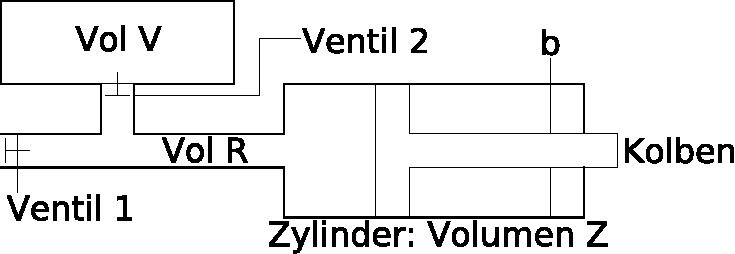
\includegraphics[width=0.8\textwidth]{include/evakuierungspumpe.pdf}
\begin{align*}
p_0: &\text{ Außendruck} \\
V: &\text{ zu evakuierendes Volumen} \\
R: &\text{ Restvolumen des Gestänges}
\end{align*}
\end{center}
%\end{minipage}

\begin{theorem}[Gasgesetz von Boyle-Mariotte]
\begin{align*}
p \cdot V = C \cdot m &&
\begin{aligned}
&p: \text{Druck} \\
&V: \text{Volumen} \\
&m: \text{Masse} \\
&C: \text{Boltzmann-Konstante}g
\end{aligned}
\end{align*}
\end{theorem}

\paragraph*{Funktionsweise}
\begin{itemize}
  \item Kolben in Stellung b; Ventil 1 offen; Ventil 2 geschlossen; d.h. Außenluft
  \item Kolben fährt nach a; Ventil 2 geschlossen; Ventil 2 geschlossen
  \item Kolben fährt nach b; Ventil 1 geschlossen; Ventil 2 offen; d.h. evakuiert V
\end{itemize}
Ergebnis: schrittweise Änderung des Drucks

\paragraph*{Modellierung}
\begin{enumerate}
	\item Kolbenhub (Stellung a)
	\begin{align*} \left.
		\begin{aligned}
			p_0 \cdot (V + R) &= C \cdot (m_v + m_r) \\
			\text{Kolben zu b} &= p_1 \cdot (V + R + Z)
		\end{aligned} \right\rangle
		p_1 = \frac{p_0 \cdot V + p_0 \cdot R}{V + R + Z}
	\end{align*}
	\item Kolbenschub
	\begin{align*}
	p_1 \cdot V + p_0 \cdot R &= p_2 \cdot (V + R + Z) && \text{Außendruck in R durch Öffnen des Ventils 1} \\
	p_2 &= \frac{p_1 \cdot V + p_0 \cdot R}{V + R + Z} \\
	&\vdots \\
	p_n &= \frac{p_{n-1} \cdot V + p_0 \cdot R}{V + R + Z} \\
	\end{align*}
\end{enumerate}
\begin{itemize} 
  \item Gibt es einen Grenzdruck $p_n \rightarrow p^*$?
  \item Auslegung von Z, R
\end{itemize}
Zahlenfolge $p_0, p_1, \ldots \rightarrow$\todo{unklar}

\end{example}

\begin{definition}[Zahlenfolge]
Eine Funktion $f: \mathbb N \rightarrow \mathbb N$ heißt reelle (Zahlen)folge.\\
Notation: $f_n$ oder $(f_n)_{n \in \mathbb N}$
\end{definition}

\begin{example}
\begin{enumerate}
	\item $a_n = n$: $a_1 = 1, a_2 = 2, \ldots$
	
\begin{tikzpicture}
	[uplabel/.style={above=4mm,anchor=center},
	 downlabel/.style={below=4mm,anchor=center}]
%\draw (0.5,0) -- (3.5,0)
% LH: scaling
\draw (0.5,0) -- (5,0)
(1,0) node (a1) {} node[uplabel] {$a_1$} node[downlabel] {1}
(2.75,0) node (a2) {} node[uplabel] {$a_2$} node[downlabel] {2}
(4.5,0) node (a3) {} node[uplabel] {$a_3$} node[downlabel] {3};
\foreach \n in {a1,a2,a3}
\draw (\n) ++(0,-0.1) -- ++(0,0.2);
\end{tikzpicture}\hspace{1cm}
\begin{tikzpicture}[line cap=round,line join=round,>=triangle 45,x=1.0cm,y=1.0cm]
\draw[color=white] (-1,0) -- (-0.5,0);
\draw[->,color=black] (-0.5,0) -- (2.5,0);
\foreach \x in {,1,2}
\draw[shift={(\x,0)},color=black] (0pt,2pt) -- (0pt,-2pt) node[below] {\footnotesize $\x$};
\draw[->,color=black] (0,-0.5) -- (0,2.5);
\foreach \y in {,1,2}
\draw[shift={(0,\y)},color=black] (2pt,0pt) -- (-2pt,0pt) node[left] {\footnotesize $\y$};
\draw[color=black] (0pt,-10pt) node[right] {\footnotesize $0$};
\clip(-0.5,-0.5) rectangle (2.5,2.5);
\fill [color=black] (1,1) circle (1.5pt);
\fill [color=black] (2,2) circle (1.5pt);
\end{tikzpicture}

	\item $a_n = \frac{1}{n}$: $a_1 = 1, a_2 = \frac{1}{2}, a_3 = \frac{1}{3}, \ldots$\label{ex:nullfolge}
	
	\begin{tikzpicture}
	[uplabel/.style={above=4mm,anchor=center},
	 downlabel/.style={below=4mm,anchor=center}]
% \draw (0.5,0) -- (3.5,0)
% LH: scaling
\draw (0.5,0) -- (5,0)
(1,0) node (n0) {}  node[downlabel] {0}
(4.5,0) node (a1) {} node[uplabel] {$a_1$} node[downlabel] {1}
(2.75,0) node (a2) {} node[uplabel] {$a_2$} node[downlabel] {$\frac{1}{2}$}
(2.17,0) node (a3) {} node[uplabel] {$a_3$} node[downlabel] {$\frac{1}{3}$};
\foreach \n in {n0, a1,a2,a3}
\draw (\n) ++(0,-0.1) -- ++(0,0.2);
\end{tikzpicture}\hspace{1cm}
\begin{tikzpicture}[line cap=round,line join=round,>=triangle 45,x=1.0cm,y=1.0cm]
\draw[color=white] (-1,0) -- (-0.5,0);
\draw[->,color=black] (-0.5,0) -- (3.5,0);
\foreach \x in {,1,2,3}
\draw[shift={(\x,0)},color=black] (0pt,2pt) -- (0pt,-2pt) node[below] {\footnotesize $\x$};
\draw[->,color=black] (0,-0.5) -- (0,1.5);
\foreach \y in {,1}
\draw[shift={(0,\y)},color=black] (2pt,0pt) -- (-2pt,0pt) node[left] {\footnotesize $\y$};
\draw[color=black] (0pt,-10pt) node[right] {\footnotesize $0$};
\clip(-0.5,-0.5) rectangle (3.5,1.5);
\fill [color=black] (1,1) circle (1.5pt);
\fill [color=black] (2,0.5) circle (1.5pt);
\fill [color=black] (3,0.33) circle (1.5pt);
\end{tikzpicture}

	\item $a_n = (-1)^n$: $a_1 = -1, a_2 = 1, \ldots$

	\begin{tikzpicture}
	[uplabel/.style={above=4mm,anchor=center},
	 downlabel/.style={below=4mm,anchor=center}]
%\draw (0.5,0) -- (3.5,0)
% LH: scaling
\draw (0.5,0) -- (5,0)
(2.75,0) node (n0) {}  node[downlabel] {0}
(1,0) node (a1) {} node[uplabel] {$a_1$}  node[downlabel] {-1}
(4.5,0) node (a2) {} node[uplabel] {$a_2$} node[downlabel] {1};
\foreach \n in {n0,a1,a2}
\draw (\n) ++(0,-0.1) -- ++(0,0.2);
\end{tikzpicture}\hspace{1cm}
\begin{tikzpicture}[line cap=round,line join=round,>=triangle 45,x=1.0cm,y=1.0cm]
\draw[color=white] (-1,0) -- (-0.5,0);
\draw[->,color=black] (-0.5,0) -- (4.5,0);
\foreach \x in {,1,2,3,4}
\draw[shift={(\x,0)},color=black] (0pt,2pt) -- (0pt,-2pt) node[below] {\footnotesize $\x$};
\draw[->,color=black] (0,-1.5) -- (0,1.5);
\foreach \y in {-1,1}
\draw[shift={(0,\y)},color=black] (2pt,0pt) -- (-2pt,0pt) node[left] {\footnotesize $\y$};
\draw[color=black] (0pt,-10pt) node[right] {\footnotesize $0$};
\clip(-0.5,-1.5) rectangle (4.5,1.5);
\fill [color=black] (1,-1) circle (1.5pt);
\fill [color=black] (2,1) circle (1.5pt);
\fill [color=black] (3,-1) circle (1.5pt);
\fill [color=black] (4,1) circle (1.5pt);
\end{tikzpicture}

\end{enumerate}
\end{example}

\paragraph*{Frage}
Streben die Folgen gegen ausgezeichnete Werte?
Im Beispiel \ref{ex:nullfolge} ist es der Null-Wert: $a_n \rightarrow 0$.\\
Zentrale Werkzeuge: Schranken und Monotonie

\begin{definition}[Beschränktheit]
Eine reelle Folge $(a_n)_{n \in \mathbb N}$ heißt nach oben beschränkt, falls ein reelles $L$ existiert mit
\begin{equation*} a_n \le L\end{equation*}
analog: nach unten beschränkt
\begin{equation*} a_n \ge L\end{equation*}
\end{definition}

\begin{example}
\begin{enumerate}
	\item untere Schranke $1$, keine obere Schranke
	\item untere Schranke $0$, obere Schranke $1$
	\item untere Schranke $-1$, obere Schranke $1$
\end{enumerate}
\end{example}

\begin{example}[Evakuierungspumpe, Fortsetzung]
Druckfolge $p_n$
\begin{itemize}
\item nach unten durch 0 beschränkt (da nur positive Terme)
\item nach oben durch $p_0$ beschränkt
\begin{align*}
p_1 &= p_0 \cdot \frac{V + R}{V + R + Z} < p_0 \\
p_2 &= \frac{p_1 \cdot V + p_0 \cdot R}{V + R + Z} < \frac{p_0 \cdot V + p_0 \cdot R}{V + R + Z} < p_0 \\
p_n &\text{ analog}
\end{align*}
\end{itemize}
\end{example}

\begin{definition}[Monotonie]
Eine reelle Folge heißt monoton wachsend, wenn $\forall n \in \mathbb N : a_n \le a_{n+1}$ und
streng monoton wachsend, wenn $a_n < a_{n+1}$. Analog: (streng) monoton fallend.
\end{definition}
Anschaulich: monoton wachsend + obere Schranke $\Rightarrow$ Grenzwert existiert $\equiv$ Supremumaxiom $\mathbb R$
\newpage
\lecture{2009-11-17}

\todo[inline]{könnte redundant zur vorheringen Vorlesung sein}
\begin{note}
 Falls eine Folge monoton und beschränkt ist, dann ist der Grenzwert die kleinste obere/untere Schranke. (Im Prinzip wäre man fertig, aber Folgen wie $a_n = \frac{(-1)^n}{n^2}$ würden nicht erfasst. $\leadsto$ Formalisierung erforderlich
\end{note}

\paragraph*{1. Schritt:} $\varepsilon$-Charakterisierung des Grenzwertes $\alpha$ \\
zu jedem $\varepsilon > 0$ ex. $n_\varepsilon$ mit $\alpha-\varepsilon < a_{n_\varepsilon}$
\paragraph*{2. Schritt:}
  \begin{equation*}
    \forall \varepsilon > 0\; \exists n_\varepsilon \;\forall n \geq n_\varepsilon: \;\left|a_n-\alpha\right| < \varepsilon
  \end{equation*}

\begin{definition}[Grenzwert]
  Eine Zahl $\alpha$ heißt Grenzwert (\emph{Limes}) einer Folge $a_n$, falls gilt:
  \begin{equation*}
    \forall \varepsilon > 0\; \exists n_\varepsilon \in \mathbb{N} \;\forall n \geq n_\varepsilon:\; \left| a_n - \alpha \right| < \varepsilon
  \end{equation*}
  Symbol: $\displaystyle\alpha = \liminfty{a_n}$\\
  Eine Folge heißt \emph{konvergent}, falls sie einen Grenzwert besitzt.
\end{definition}

\begin{note}[rekursiv definierte Folge]
  das $n$-te Folgenelement berechnet sich aus den Vorgängern
\end{note}

\begin{example}[rekursiv definierte Folge]
  Evakuierungspumpe: $p_n$ aus $p_{n-1}$ und $p_0$
\end{example}

\begin{note}[Grenzwert in drei Schritten]
  \begin{enumerate}
   \item beschränkt
   \item monoton
   \item Grenzwert berechnen durch Einsetzen $\displaystyle p^\ast = \liminfty{p_n}$
  \end{enumerate}
\end{note}

\begin{example}[Evakuierungspumpe]
  \[ p_n = \frac{p_{n-1}V+p_0R}{V+R+Z} \]
  \begin{enumerate}
    \item nach unten durch $0$ beschränkt
    \item monoton fallende Folge
    \item[$\Rightarrow$] es existiert ein Infimum $\inf p_n$ $\equals$ Grenzwert
    \item
      \begin{equation*}
        \liminfty{p_n} = \frac{\liminfty{p_{n-1}V}+p_0R}{V+R+Z} \Rightarrow
        p^\ast = \frac{p^\ast V+p_0R}{V+R+Z} = \frac{p_0R}{R+Z}
      \end{equation*}
  \end{enumerate}
\end{example}

\subsubsection*{Begriffe}

\emph{Konvergenz} -- es existiert ein Grenzwert\\
\emph{Divergenz} -- es existiert kein Grenzwert\\
\emph{Nullfolge} -- es existiert ein Grenzwert, dieser ist $0$

\subsubsection*{Rechenregeln für Nullfolgen}

\begin{note}
  konvergente Folge $a_n$ mit Grenzwert $\alpha \neq 0$ kann in Nullfolge transformiert werden: $b_n = a_n - \alpha$ ist Nullfolge
\end{note}

\begin{enumerate}
  \item $a_n, b_n$ Nullfolgen $\Rightarrow$ $a_n+b_n$ Nullfolge
  \item $a_n$ Nullfolge, $b_n$ beschränkt $\Rightarrow$ $a_n\cdot b_n$ Nullfolge
  \item $\left|b_n\right| < \left|a_n\right|$, $a_n$ Nullfolge  $\Rightarrow$ $b_n$ Nullfolge
\end{enumerate}

\begin{lemma}[Eindeutigkeit des Grenzwerts]
  Jede Folge $a_n$ hat höchstens einen Grenzwert.
\end{lemma}
\begin{proof}
  Angenommen, es existieren zwei Grenzwerte $\widehat a$ und $\overline a$, dann gilt nach Definition:
  \begin{align*}
    \left| a_n - \widehat a \right| &< \varepsilon \text{ für alle $n \geq N_1(\varepsilon)$} \\
    \left| a_n - \overline a \right| &< \varepsilon \text{ für alle $n \geq N_2(\varepsilon)$}
    \intertext{wähle $n \geq \max(N_1(\varepsilon),N_2(\varepsilon))$}
    \left| \widehat a - \overline a \right| &= \left| \widehat a - a_n + a_n - \overline a \right| \\
    & \leq \underbrace{\left| \widehat a - a_n \right|}_{< \varepsilon} + \underbrace{\left| a_n - \overline a \right|}_{< \varepsilon} \\
    & < \varepsilon + \varepsilon = 2\varepsilon
  \end{align*}
  $\Rightarrow \overline a = \widehat a$, da $\varepsilon$ beliebig klein aber $> 0$
\end{proof}

\begin{example}[Anwendungen]
\begin{enumerate}
  \item\label{ex:polynomlimes}
    \[
      \liminfty{x^n} = \begin{cases}
                          0 & \text{für $\left|x\right| < 1$ (Nullfolge)} \\
                          1 & \text{für $x=1$} \\
                          \infty & \text{für $x>1$} \\
                          \text{unbest.} & \text{für $x \leq -1$}
                       \end{cases}
    \]
  \item
    \begin{align*}
      a_n = \sqrt{n+1} - \sqrt n &\xrightarrow[n \rightarrow \infty]{} \infty - \infty = \text{?}\\
      &= \frac{(\sqrt{n+1}-\sqrt n)(\sqrt{n+1}+\sqrt n)}{\sqrt{n+1}+\sqrt n}\\
      &= \frac{n+1-n}{\sqrt{n+1}+\sqrt n}\\
      &= \frac 1 {\sqrt{n+1} + \sqrt n}\\
      &\xrightarrow[n \rightarrow \infty]{} 0
    \end{align*}
  \item geometrische Reihe
    \begin{equation*}
      s_n = 1 + x + \ldots + x^n = \begin{cases}
                                     \frac{1-x^{n+1}}{1-x} & \text{ für } x \neq 1 \\
                                     n + 1 & \text{ für } x = 1
                                   \end{cases}
    \end{equation*}
    aus Beispiel \ref{ex:polynomlimes}: nur konvergent für $\left| x \right| < 1$\\
    für $\left| x \right| < 1$:
    \begin{equation*}
      \liminfty{s_n} = \liminfty{\frac{1-x^{n+1}}{1-x}} = \frac{1-\displaystyle\liminfty{x^{n+1}}}{1-x} = \frac 1 {1-x}
    \end{equation*}
  \item harmonische Reihe\\
    Folge $s_n = \displaystyle 1 + \frac 1 2 + \frac 1 3 + \ldots + \frac 1 n$ ist divergent, denn
    \begin{align*}
      s_{2k+1} &= 1 + \frac 1 2 + \left( \frac 1 3 + \frac 1 4 \right) + \left( \frac 1 5 + \ldots \frac 1 8 \right) + \ldots + \left(\frac 1 {2^k+1} + \ldots + \frac 1 {2^{k+1}}\right) \\
      &\geq 1 + \frac 1 2 + 2 \cdot \frac 1 4 + 4 \cdot \frac 1 8 + \ldots + 2^k \cdot\frac 1 {2^{k+1}}\\
      &= \frac{k+3} 2 \\
      \Rightarrow \liminfty[k]{s_{2k+1}} &= \infty
    \end{align*}
    %
    \begin{note}
      Mantissenlänge (Zahldarstellung) und Taktzahl müssen so abgestimmt sein, dass ein unerfahrenere Nutzer in ca. 1 Tag Rechenzeit keine Konvergenz der harmonsichen Reihe erzielt (bisheriger Standard $R \ast 8$ nicht mehr ausreichend).
    \end{note}
  \item Eulersche Zahl $\euler = 2,71828\ldots$
    \begin{equation*}
      \euler := \sum\limits_{k=0}^\infty \left( \frac 1 {k!} \right) \rightarrow \text{ Grenzwert der Zahlenfolge}
    \end{equation*}
    \begin{enumerate}
      \item nach oben beschränkt
        \begin{align*}
          0 &\leq 1 + \frac 1 {1!} + \ldots + \frac 1 {n!} \\
          &\leq 1+1+\frac 1 2 + \ldots + \frac 1 {2^n}
        \end{align*}
      \item monoton wachsend
        \begin{equation*}
          b_{n+1} = 1 + \frac 1 {1!} + \ldots + \frac 1 {(n+1)!} = b_n + \frac 1 {(n+1)!} > b_n
        \end{equation*}
      \item[$\Rightarrow$] konvergent, Grenzwert $\leq 3$
    \end{enumerate}

\end{enumerate}

\end{example}

\newpage
\addcontentsline{toc}{chapter}{Literaturverzeichnis}
\bibliography{bibliography}

\end{document}
